\documentclass{these}
\usepackage[french]{babel}
\usepackage[utf8]{inputenc} 
\usepackage[T1]{fontenc}
\usepackage{lmodern}
\usepackage[babel=true]{csquotes}
\usepackage{lscape}
\usepackage{amssymb}
\usepackage{chngpage}
\usepackage{chngcntr}

% Informations factuelles
\title{\huge Analyse et intégration de techniques \enquote{constraint programming} et \enquote{operations research} pour la réalisation d'un outil d'aide à la création d'horaires}
\author{Kevin \textsc{Jacoby} et Xavier \textsc{Dubruille}}
\date{2012}
\labo{CENTAL}
\school{École Doctorale}
\speciality{Traitement Automatique du Langage}
\university{Linguistique à Finalité TAL}{Ecole Pratique des Hautes Etudes Commerciales}
%\ISBN{} %à remplir et décommenter lorsque ce numéro est connu.
\advisor[M]{C. \bsc{Lambeau}} %Directeur de thèse


% Compteur de figure
\counterwithout{figure}{chapter}
\counterwithout{table}{chapter}


% Profondeur TOC
\setcounter{tocdepth}{1}
\stepcounter{secnumdepth}
\stepcounter{tocdepth}


% Références
\usepackage[colorlinks=false]{hyperref}
\hypersetup{urlcolor=black,linkcolor=black,citecolor=black,colorlinks=true}
%\usepackage[pdftex, pdfborder={0 0 0},hypertex]{hyperref}

% Math
\everymath{\displaystyle}

% Code
\usepackage[dvipsnames]{xcolor}
\usepackage{listings}
\lstset{% general command to set parameter(s)
language=SQL,
basicstyle=\small,
% print whole listing small
keywordstyle=\color{violet}\bfseries\bf,
% underlined bold black keywords
identifierstyle=\color{blue},
% nothing happens
commentstyle=\color{red}\bf, % white comments
stringstyle=\ttfamily,
% typewriter type for strings
showstringspaces=false}

% Pstree
%\usepackage{pstricks}
%\usepackage{pst-plot,pst-text,pst-tree,pst-eps,pst-fill,pst-node,pst-math}
%\usepackage[on]{auto-pst-pdf} 
%\def\TTR{\Tr{\Tcircle[fillstyle=solid,fillcolor=black!60]%
%  {}}}
  
% Paragraph
\makeatletter
\renewcommand{\paragraph}{\@startsection{paragraph}{4}{0ex}%
   {-3.25ex plus -1ex minus -0.2ex}%
   {1.5ex plus 0.2ex}%
   {\normalfont\normalsize\bfseries}}
\makeatother

% Page vierge après Part
\makeatletter
\renewcommand{\@endpart}{\vfil\newpage\if@tempswa\twocolumn\fi}
\makeatother

%Nospace
\makeatletter
\@ifpackageloaded{babel}%
        {\newcommand{\nospace}[1]{{\NoAutoSpaceBeforeFDP{}#1}}}%  % !! double {{}} pour cantonner l'effet à l'argument #1 !!
        {\newcommand{\nospace}[1]{#1}}
\makeatother

% Citation - Bibliographie
\usepackage{natbib}
\bibpunct{(}{)}{;}{a}{}{;} 

% Intégration d'images
\usepackage{graphicx}
%\graphicspath{{./pics/}} 

% Siècle
\def\siecle#1{\textsc{\romannumeral #1}\textsuperscript{e}~siècle}

%%%%%%%%%%%%%%%%%%%%%%%%%%%%%%
% Document
%%%%%%%%%%%%%%%%%%%%%%%%%%%%%%
\begin{document}

% Titre
\frontmatter
\maketitle


\maketitle
%\setcounter{page}{6} 

%%%%%%%%%%%%%%%%%%%%%%%%%%%%%%
% Resume
%%%%%%%%%%%%%%%%%%%%%%%%%%%%%%
% !TeX root = these.tex
\resume{
Un abstract présente en 100-150 mots
la substantifique moelle du travail.\\

    l'intérêt de la question\\
    la problématique\\
    quelques mots de méthodologie\\
    les résultats principaux\\
    quelques conclusions et leurs implications\\

Un abstract :\\

    N'est pas un résumé du travail.\\

    Ne dit pas tout ce que le travail contient.\\

    Ne développe pas toute l'argumentation et l'analyse de la recherche...\\

    Ne dit pas tout mais donne envie de lire.\\

\noindent
\Large
\textbf{Mots-clefs }\normalsize \textbf{:} constraint programming, operations research, horaire de cours

}{}

%%%%%%%%%%%%%%%%%%%%%%%%%%%%%%
% Remerciements
%%%%%%%%%%%%%%%%%%%%%%%%%%%%%%
% !TeX root = these.tex

\newpage
\chapter*{Avant-propos}
En préambule à ce mémoire, nous souhaitons adresser nos remerciements les plus sincères aux personnes qui nous ont apporté
leur aide et qui ont contribué à l'élaboration de ce mémoire.\\
\newline
\indent
Nous tenons à remercier chaleureusement:
\begin{itemize}
\item Monsieur Lambeau, notre promoteur, pour le temps qu'il a bien voulu nous consacrer et sans qui ce mémoire n'aurait jamais vu le jour\\

\item Monsieur Fauconnier, pour la grande patience dont il a su faire preuve et le temps précieux qu'il nous a accordé\\
%      \item Monsieur François Henry, notre assistant en thermodynamique, qui a accepté de répondre à nos questions avec gentillesse,
\item Madame Bonnave qui a eu la gentillesse de relire et corriger ce travail.\\
\end{itemize}

%%%%%%%%%%%%%%%%%%%%%%%%%%%%%%
% TOC
%%%%%%%%%%%%%%%%%%%%%%%%%%%%%%
\newpage
\tableofcontents

%%%%%%%%%%%%%%%%%%%%%%%%%%%%%%
% Abréviation
%%%%%%%%%%%%%%%%%%%%%%%%%%%%%%
\newpage
%% !TeX root = these.tex

\chapter*{Liste des abréviations}

\begin{tabular}{l l}
\textbf{ASCII} & American Standard Code for Information Interchange\\
\textbf{CERN} & European Organization for Nuclear Research\\
\textbf{DEC} & Digital Equipment Corporation\\
\textbf{DNS} & Domain Name System\\
\textbf{DTD} & Document Type Definition\\
\textbf{FAI} & Fournisseur d'Accès à Internet\\
\textbf{FTP} & File Transfer Protocol\\
\textbf{HTTP} & Hypertext Transfer Protocol\\
\textbf{IA} & Intelligence Artificielle\\
\textbf{IBM} & International Business Machines\\
\textbf{ICANN} & Internet Corporation for Assigned Names and Numbers\\
\textbf{IC} & Ingénierie des Connaissances\\
\textbf{IETF} & Internet Engineering Task Force\\
\textbf{IRI} & Internationalized Resource Identifier\\
\textbf{ISP} & Internet Service Provider\\
\textbf{OWL} & Web Ontology Language\\
\textbf{RDF} & Resource Description Framework\\
\textbf{RDFS} & RDF Schema\\
\textbf{RFC} & Requests for Comments\\
\textbf{RI} & Recherche d'Information\\
\textbf{SBC} & Système à Base de Connaissances\\
\textbf{SGBD} & Système de Gestion de Base de Données\\
\textbf{SGML} & Standard Generalized Markup Language\\
\textbf{SPARQL} & SPARQL Protocol and RDF Query Language\\
\textbf{SQL} & Structured Query Language\\
\textbf{SRI} & Système de Recherche d'Information\\
\textbf{TREC} & Text REtrieval Conference\\
\textbf{UML} & Unified Modeling Language\\
\textbf{URI} & Uniform Resource Identifier\\
\textbf{URL} & Uniform Resource Locator\\
\textbf{URN} & Uniform Resource Name\\
\textbf{W3C} & World Wide Web Consortium\\
\textbf{XML} & Extensible Markup Language\\
\end{tabular}








%%%%%%%%%%%%%%%%%%%%%%%%%%%%%%
% Debut du document
%%%%%%%%%%%%%%%%%%%%%%%%%%%%%%
\newpage
\mainmatter
% !TeX root = these.tex


\chapter*{Introduction}
%étapes traditionnellement dans l’introduction :
%• l’accroche, 1) capter l’attention du lecteur
%• la problématique 2) délimiter le sujet
%• l’annonce du plan (très claire) 3) annoncer le plan

Dans le domaine de l'enseignement, la création des horaires de cours est une tâche ardue pour les secrétariats. En effet, il s'agit de prendre simultanément en compte de très nombreuses contraintes ; les locaux ne sont pas toujours libres, les professeurs ont des \textit{desideratas} particuliers, les élèves ont des parcours différents, etc. Cette somme de critères contraignants font de la mise en place d'emplois du temps pour chacun des professeurs et, corollairement, des élèves, un travail long et fastidieux qui doit être réitéré à chaque rentrée académique.\\
\newline
\indent
Ce type de problème est l'objet de la programmation par contraintes, dite \enquote{constraint programming} \citep{Muller_2005}. Ce paradigme de programmation s'attache à traiter les problèmes où une large combinatoire est nécessaire pour trouver un ensemble de solutions satisfaisant les différents acteurs impliqués. Par exemple, la programmation par contraintes est notamment utilisée pour traiter les problèmes relatifs aux circuits d'attente aérien au-dessus des aéroports. Il s'agit de prendre simultanément en compte la quantité de kérosène restante pour chacun des avions, les pistes occupées, les prédictions météos, les \enquote{gates} libres, les ressources disponibles au sol, etc. Mais, la programmation par contraintes se retrouve aussi dans d'autres tâches telles que la gestion de la main d’œuvre, la mise en place de tournois sportifs de grande envergure, etc.
\newline
\indent
La recherche par contrainte constitue l'un des outils fondamentaux du domaine, plus vaste, de la 
recherche opérationnelle, dite \enquote{operations research} \citep{Scharlig_1985}. La recherche opérationnelle se donne pour objectif d'aider la prise de décision pour trouver une solution optimale face à un problème donné. Dans ce contexte, il est naturel que la programmation par contraintes, par sa prise en compte de critères multiples, trouve sa place comme méthode de résolution de problèmes.\\
\newline
\indent
C'est dans ce contexte que s'inscrit le présent travail qui vise à détailler la procédure de conception d'un outil dédié à la création d'horaires de cours pour l'EPHEC\footnote{Ecole Pratique des Hautes Etudes Commerciales} et reposant sur la programmation par contraintes.
\newline
\indent
Madame \textsc{Gillet}, Directrice de l'établissement EPHEC à Louvain-la-Neuve, établit l'horaire à chaque nouveau semestre de l'année académique. L'établissement de cet horaire nécessite de considérer un grand nombre de contraintes ; citons notamment les \textit{desideratas} exprimés par les professeurs, la nécessité qu'un cours se donne dans un local avec un matériel adapté au sujet qu'il traite\footnote{Par exemple, certains cours nécessitent du matériel informatique pour leur bonne tenue.} ou, encore, les impératifs liés au programme de cours des différentes promotions.
\newline
\indent
Toutefois, dans le cadre particulier de l'EPHEC, certaines difficultés supplémentaires sont à examiner. En effet, les professeurs externes, qui ont des charges d'enseignements dans d'autres établissements, doivent se voir attribuer des horaires spécifiques.  De plus, certains cours sont dispensés dans des locaux hors des murs de l'EPHEC qui ont des périodes de disponibilité variables qu'il est nécessaire de prendre en compte.\\
\newline
\indent
Sans une approche computationnelle, ces contraintes doivent être  être prises en compte manuellement par la personne établissant l'horaire. Or, cette considération minutieuse des contraintes est un véritable \enquote{casse-tête} nécessitant un effort cognitif important pour le résoudre. 
\newline
\indent
La programmation par contraintes permet de résoudre de manière automatique cette problématique et facilite ainsi la tâche qui incombe à la personne en charge de l'élaboration d'un horaire. Ainsi, notre solution s'inscrit dans un cadre applicatif réel et  utile face à la tâche chronophage de création d'horaires. \\
\newline
\indent
Afin de répondre à cette problématique, différents aspects ont dû être étudiés ; la notion de contrainte que nous décrirons de façon théorique, le paradigme de programmation correspondant et, enfin,  les différents outils existants dédiés à ce domaine. Cependant, afin de rendre notre solution utile au plus grand nombre, deux aspects supplémentaires ont du être travaillés.
\newline
\indent
Premièrement, il a été décidé d'orienter notre solution dans une visée de service Web. Ainsi, notre solution ne nécessite pas d'installation préalable à son utilisation. Et, en outre, ce choix permet de centraliser les données au sein d'une unique base de données.
\newline
\indent
Deuxièmement, dans une optique d'ergonomie et de facilité d'emploi, il a été choisi d'effectuer un travail important sur l'interface. En effet, la création d'horaires étant une tâche déjà complexe en soi, il nous a paru inutile d'alourdir la charge cognitive qu'elle nécessite en obligeant l'utilisateur à apprendre à manipuler notre solution.\\
\newline
\indent
Ces deux aspects ont apportés un lot de difficultés auquel notre solution a dû répondre. Citons notamment la nécessité d'une approche asynchrone dans la gestion de la base de données afin de garder une solution rapide. En effet, lorsqu'un horaire subit une modification, il est nécessaire de le changer dans le base de donnée. Cette demande faite à la base de données nécessite une réponse avant de pouvoir continuer. Or, le temps de réponse, au vu des traitements nécessaires, n'est pas toujours  assez rapide. En conséquence, il a été nécessaire d'utiliser des fonctions de rappel, dit \enquote{callback}, afin de ne pas ralentir l'ensemble du système.
\newline
\indent
De plus, la mise en place d'un service Web a aussi apporté la nécessité d'utiliser des librairies avancées. Par exemple, nous faisons un grand usage de Google Web Toolkit et Java EE. Ces deux outils proposent des méthodes orientées service Web, cependant, ils nécessitent un temps d'apprentissage plus long comparé à des solutions basiques.
\newline
\indent
D'autres difficultés ont été rencontrées au cours de notre travail et seront explicitées dans le suite de ce travail.\\
\newline
\indent
Afin d'étayer notre propos, ce présent travail se divise en sept sections :
\begin{itemize}
\item \textbf{La première section} présente la solution dans son ensemble. Y sont notamment décrits l'interface, l'implémentation effective des contraintes, l'utilisation de la mémoire cache, etc.\\

\item \textbf{La deuxième section} expose le cadre technologique utilisé pour notre solution.\\

\item \textbf{La troisième section} décrit la méthodologie sous-jacente à la conception de notre solution. Y sont notamment examinés l'approche en travail d'équipe et les outils nécessaires à cette approche.\\

\item \textbf{La quatrième section} offre une présentation plus poussées des outils utilisés.\\

\item \textbf{La cinquième section} montre les différents points importants dans notre code et dans la gestion de la base de données.\\

\item \textbf{La sixième section} se destine à la programmation par contraintes et à l'implémentation qui en est faite au sein du code.\\

\item \textbf{La septième section} propose quelques réflexions sur notre solution et présente des perspectives d'extension à notre travail.\\

\end{itemize}

Enfin, une conclusion achèvera ce travail et seront synthétisés les différents aspects saillants de notre solution.




%Nous allons d'abord définir ce qu'est une contraintes de manière plus théorique pour bien saisir la problématique et la provenance de celle-ci. Nous discuterons ensuite autour des différentes solutions existantes nous permettant de réaliser cela.
%Face à ce constat, de nombreux travaux ont eu pour sujet la \enquote{constraint programming}. 
%\newline
%\indent
%L'objectif de notre mémoire est d'aider à la création des horaires de l'EPHEC.
%Dans cet objectif, nous avons décidé de créer une application internet permettant d'accéder
%aux données présentes sur les serveurs de l'école.\\
%\newline
%\indent
%Cette application est créée pour être utilisée au sein de l'école, c'est pourquoi il faut un 
%outil adapté à l'EPHEC simple d'utilisation et interactif. \\
%\newline
%\indent
%Ce rapport décrira la méthodologie utilisée et les choix de conception faits.
%Par la suite, nous décrirons plus profondément le programme et sa structure avant de clore sur une discussion sur les possibilités du programme. 


%Avant tout, il est nécessaire de bien saisir la problématique et en quoi celle-ci peut être utile à notre travail. Nous avons du faire un analyse approfondie sur ce qu'était une contraintes ainsi que la programmation de celles-ci. Il a fallu ensuite analyser les différents outils nous permettant de "programmer par contraintes" et ensuite essayer de les implémenter dans un logiciel d'aide à la création d'horaire que nous avons du créer au préalable.\\




% analyse de la problematique ainsi que les objectifs
% !TeX root = these.tex

\chapter{Analyse de la problématique et outils existants}
%Avant tout, il est nécessaire de bien saisir la problématique et en quoi celle-ci peut être utile à notre travail. Nous avons du faire un analyse approfondie sur ce qu'était une contraintes ainsi que la programmation de celles-ci. Il a fallu ensuite analyser les différents outils nous permettant de "programmer par contraintes" et ensuite essayer de les implémenter dans un logiciel d'aide à la création d'horaire que nous avons du créer au préalable.\\
%\newline
%\indent
%D'abord, pourquoi on a fait ça et pourquoi ce TFE. En quoi c'est utilite pr notre travail
%Madame Gillet, Directrice de l'établissement EPHEC à Louvain-la-Neuve, établit l'horaire a chaque nouveau quadrimestre de l'année scolaire. l'établissement d'un horaire doit se faire sous certaines contraintes et en fonction de désidératas remis par les professeurs. Le nombre de locaux informatique est limité, certains professeurs sont dit "externe" à l'EPHEC, ceux-ci doivent se voir attribué un horaire particulier, certain cours se donne dans des locaux externes à l'EPHEC et ne sont donc pas disponible à chaque période de cours. Toute ces contraintes, si elle ne sont pas informatisée doivent prise en compte par la personne établissant l'horaire qui doit réaliser un "vrai casse tête chinois" afin d'avoir un horaire le plus adéquat possible.\\
%\newline
%\indent
%La programmation par contrainte permet de résoudre de manière automatique cette problématique, facilitant ainsi la tâche qui incombe à la personne en charge de l'élaboration d'un horaire. Nous allons d'abord définir ce qu'est une contraintes de manière plus théorique pour bien saisir la problématique et la provenance de celle-ci. Nous discuterons ensuite autour des différentes solutions existantes nous permettant de réaliser cela.

%Parler de notre rencontre avec Pierre bidule je sais plus quoi
%je sais plus ce qu'on avais dit d'autre

Afin de mieux comprendre la problématique liée à l'élaboration d'un horaire, nous avons tout d'abord pris rendez-vous avec Madame \textsc{Gillet}, directrice de l'EPHEC. Madame \textsc{Gillet} est la personne en charge de l'élaboration des horaires pour la partie Louvain-la-Neuve de l'EPHEC. Nous avons parcouru ensemble les différents problèmes et les différents types de contraintes auxquelles nous devrons faire face. Cette première analyse du problème avait pour but de nous orienter sur le type de contraintes intervenant dans notre travail.
\newline
\indent
Dans un premier temps, cette présente section, théorisera la notion de contrainte. Dans un deuxième temps, seront présentées les différentes contraintes rencontrées dans l'analyse du problème. 

\section{Une contrainte en théorie}
Dans le cadre d'un horaire, nous devons faire face à des contraintes sur des domaines finis. Nous allons illustrer ce concept comme suite :
\begin{center}
$P=(X,D,C)$
\end{center}

$X$ étant nos variables. Celles-ci seront représentées par les attributions\footnote{Les attributions sont les différents cours avec leurs propriétés intrinsèques. Dans le cadre de ce rapport, nous désignerons ces cours par l'appellation de cartons. Cette notion sera explicitée plus loin dans le présent rapport.} dans lesquelles nous retrouverons les éléments suivants :
\begin{itemize}
\item nom du professeur
\item le cours
\item la classe
\end{itemize}
Nous pouvons l'écrire sous la forme $Vn$ ou $V$ correspond à la valeur du carton, et n sont numéro.\\
\newline
\indent
	$D$ correspond au domaine. Ici, il s'agit d'effectuer un horaire. Notre domaine sera le nombre de locaux disponibles multiplié par le nombre de périodes. Dans le cadre du cours du jour à l'EPHEC de Louvain-la-Neuve, nous avons 6 périodes par jour, durant 5 jours. Un local est donc disponible à 6 moments de la journée durant 5 jours/semaine. Il faut donc multiplier le nombre de local par 30. Ce domaine s'écrit donc sous la forme $Nl x Np$.
\newline
\indent
	$C$ étant nos contraintes. Il existe différents types de contraintes. Dans la section suivante, nous en énumérerons certaines pour bien se rendre compte du nombre important de celles-ci et dans quel moment elles interviennent.\\
\newline
\indent
Pour régler ce problème de contraintes, il est avantageux de prendre en compte certaines heuristiques ou métaheuristiques. Nous avons défini le problème rencontré à l'EPHEC comme  étant de type NP-Complet.
\newline
\indent
La problématique de la programmation par contrainte est que les algorithmes de résolution tentent à trouver une solution \texttt{optimale} au problème. Si une contrainte ne peut être prise en compte lors de cette tentative, nous n'obtiendrons pas de résultat. Pour ce faire, il est nécessaire d'appliquer un filtrage de ce qui ne peut être pris en compte. Ce \enquote{mécanisme} s'appelle la \texttt{propagation de contraintes}.
\newline
\indent
La propagation de contraintes a pour objectif d'appliquer un filtrage sur les attributions posant problèmes et de les retirer du pool de cartons\footnote{Le pool de cartons présente l'ensemble des cours qu'il est possible de positionner dans le semainier. Cette notion de pool de cartons sera vue dans le prochain chapitre.} pris en charge lors de la résolution de l'horaire. Il est nécessaire de prendre en compte le temps que le filtrage va prendre afin de garantir une meilleure rapidité de la résolution.

\section{Les types de contraintes}

Pour se rendre compte de l'ensemble des contraintes à prendre en compte lors de l'établissement de l'horaire, nous en avons énuméré un maximum dont voici la liste :\\

\begin{table}[h!]
\begin{minipage}[t]{.3\linewidth}
    \begin{tabular}{|l|}
    \hline
\textbf{Locaux}\\
\hline
\hline
Matériels: (transparent, audio, Projecteur)\\
\hline
Type de local (sale info, auditoire, TP)\\
\hline
Nombres de places disponibles\\
\hline
Situation géographique \\
\hline
Attribution aux classes d'élèves\\
\hline
Marie Curie Ou Place des Sciences\\
\hline   
    \end{tabular}
\end{minipage}
\hfill
\begin{minipage}[t]{.4\linewidth}
    \begin{tabular}{|l|}
    \hline
\textbf{Professeurs}\\
\hline
\hline
Desiderata\\
\hline
Statut (externe, plein temps, ...)\\
\hline
Local où se donne le cours\\
\hline
Exigences matérielles\\
\hline
Pas d'enfants dans la classe\\
\hline
Temps Louvain-la-Neuve ou Bruxelles\\
\hline
    \end{tabular}
\end{minipage}
%\caption{\texttt{datatypes properties} appelées pour la description des types \textit{MusicGenre}, \textit{RecordLabel} et \textit{Settlement}}
\caption{Contraintes sur les locaux et les professeurs}
\label{locaux_prof}
\end{table}

\begin{table}[h!]
\begin{minipage}[t]{.3\linewidth}
\begin{tabular}{|l|}
\hline 
\textbf{Cours}\\
\hline
\hline
Étalement dans le temps\\
\hline
Cours qui se suivent obligatoirement (ex : TP)\\
\hline
Cours qui ne doivent pas se suivre (ex: AN+NDLS)\\
\hline
Groupe ou demi-groupe\\
\hline
Nombre d'heures total\\
\hline
Hebdomadaire ou bimensuel\\
\hline
\end{tabular}
\end{minipage}
\hfill
\begin{minipage}[t]{.4\linewidth}
\begin{tabular}{|l|}
\hline 
\textbf{Attribution (ou carton)}\\
\hline
\hline
Doit pouvoir ignorer les contraintes\\
\hline
Doit pouvoir ajouter des contraintes\\
\hline
\end{tabular}
\end{minipage}
%\caption{\texttt{datatypes properties} appelées pour la description des types \textit{MusicGenre}, \textit{RecordLabel} et \textit{Settlement}}
\caption{Contraintes sur les cours et les attributions}
\label{cours_attribution}
\end{table}

%\begin{center}
%\begin{tabular}{|l|}
%\hline 
%\textbf{Cours}\\
%\hline
%\hline
%Étalement dans le temps\\
%\hline
%Cours qui se suivent obligatoirement (ex : TP)\\
%\hline
%Cours qui ne doivent pas se suivre (ex: AN+NDLS)\\
%\hline
%Groupe ou demi-groupe\\
%\hline
%Nombre d'heures total\\
%\hline
%Hebdomadaire ou bimensuel\\
%\hline
%\end{tabular}
%\end{center}
%\bigskip
%
%
%\begin{center}
%\begin{tabular}{|l|}
%\hline 
%\textbf{Attribution (ou carton)}\\
%\hline
%\hline
%Doit pouvoir ignorer les contraintes\\
%\hline
%Doit pouvoir ajouter des contraintes\\
%\hline
%\end{tabular}
%\end{center}

\newpage

\begin{table}[!h]
\begin{center}
\begin{tabular}{|p{\linewidth}|}
\hline 
\textbf{Contraintes générales}\\
\hline
\hline
Éviter les heures de fourches\\
\hline
Si possible, garder les élèves dans un même local et faire déplacer le professeur\\
\hline
Ordre sur les contraintes (poids sur celle-ci) afin de favoriser un externe plutôt qu'un interne\\
\hline
Attribuer les locaux informatiques à un jour donné pour une option\\
\hline
Séparer eu deux semestres\\
\hline
Prendre en compte les jours de congé\\
\hline
Directrice doit définir demi-classe, groupe, etc. pour un cours\\
\hline
Il doit être possible de reporter un cours\\
\hline
Il doit être possible de définir une pause\\
\hline
\end{tabular}
\end{center}
\caption{Contraintes générales}
\end{table}
\bigskip


Pour des améliorations futures, d'autres contraintes pourront éventuellement être prises en charge comme :\\

\begin{table}[h!]
\begin{minipage}[t]{.3\linewidth}
\begin{tabular}{|l|}
\hline 
\textbf{Étudiants}\\
\hline
\hline
Répartition en fonction du sexe (sauf TI)\\
\hline
Répartition en fonction de la provenance\\
\hline
Possibilité de changer de classe\\
\hline
\end{tabular}
\end{minipage}
\hfill
\begin{minipage}[t]{.4\linewidth}
\begin{tabular}{|l|}
\hline 
\textbf{Classes}\\
\hline
\hline
Nombre d'étudiants maximum\\
\hline
Locaux adaptés\\
\hline
\end{tabular}
\end{minipage}

\caption{Contraintes sur les étudiants et les classes}
\label{etudiant_classes}
\end{table}
\bigskip



En conclusion, nous pouvons voir que le nombre de contraintes à prendre en compte pose un réel problème quand elles doivent être traitées par un humain. Les possibilités, les préférences sur certains types de contraintes devant être absolument prises en compte ou pas, relève d'une réflexion de haut niveau. Les ordinateurs "réfléchissant" de manière plus "mathématique" son en théorie plus apte à répondre de ce genre de problème.

\section{Analyse des applications existantes}
Nous avons fait également une petite étude sur les applications déjà existantes permettant d'élaborer des horaires avec contraintes. Nous pouvons citer \texttt{EDT}, programme très repandu dans les écoles, \texttt{aSc} Horaire possédant une partie automatisée et manuelle pour la création d'horaire ainsi que \texttt{Université time tabling} (UniTime). Cette dernière est une application très prometteuse, mais ne propose que l'établissement d'horaire automatique. Aucune façon manuelle de faire n'est proposée. Il utilise sa propre librairie pour résoudre la problématique des contraintes.

\section{La programmation par contraintes}
Nous avons abordé les contraintes de manière théorique, les avons énumérées et cité les applications déjà existantes, qu'en est-il de l'application de cette théorie? Pour pouvoir programmer par contraintes il existe plusieurs libraire. Certaines propriétaires et d'autres open source. Notre travail ayant pour objectif d'être libre et open source, nous nous sommes intéressés à ces dernières et en avons testé certaines :\\
\begin{itemize}
\item GeCode
\item Google OR tools
\item Python Constraint
\end{itemize}
\bigskip

Python constraint, constitue une bonne approche de la problématique, le code étant clair et concis. Celui-ci sera le plus parlant pour illustrer la programmation par contrainte de manière plus concrète.

\begin{figure}[!h]
\begin{lstlisting}[frame=single]
 from constraint import *
 problem = Problem()
 problem.addVariable("a", [1,2,3])
 problem.addVariable("b", [4,5,6])
 problem.getSolutions()
[{'a': 3, 'b': 6}, {'a': 3, 'b': 5}, {'a': 3, 'b': 4},
 {'a': 2, 'b': 6}, {'a': 2, 'b': 5}, {'a': 2, 'b': 4},
 {'a': 1, 'b': 6}, {'a': 1, 'b': 5}, {'a': 1, 'b': 4}]

 problem.addConstraint(lambda a, b: a*2 == b,
                          ("a", "b"))
 problem.getSolutions()
[{'a': 3, 'b': 6}, {'a': 2, 'b': 4}]

 problem = Problem()
 problem.addVariables(["a", "b"], [1, 2, 3])
 problem.addConstraint(AllDifferentConstraint())
 problem.getSolutions()
[{'a': 3, 'b': 2}, {'a': 3, 'b': 1}, {'a': 2, 'b': 3},
 {'a': 2, 'b': 1}, {'a': 1, 'b': 2}, {'a': 1, 'b': 3}]
\end{lstlisting}
\caption{\label{sql1}Script SQL pour la création de la table \textit{band}}
\end{figure}

\textbf{Debug : Mettre une explication du code ici}\\

Dans le cadre de notre solution, nous avons utilisé \texttt{GeCode} et \texttt{Google OR tools}. Ces deux outils sont très puissants et nous ont permis de répondre dans une certaine mesure aux contraintes explicitées.

\section{Rencontre}
Dans le cadre de ce travail, nous avons eu l'occasion de rencontrer monsieur Pierre \textsc{Schaus} qui a effectué une thèse de doctorat à l'UCL sur la problématique des contraintes. Notre rencontre nous a permis de mieux cerner la problématique.
\newline
\indent
Suite à cet entretien, nous avons pu mieux nous rendre compte de la problématique et des vigilances à prendre lors de la programmation par contraintes. Le solveur ne se contente pas d'être une librairie dans laquelle il suffirait d'appeler des fonctions pour résoudre un problème et avoir un résultat. Les choses doivent se faire petit à petit, car si le solveur ne trouve pas de résultat, il n'est pas possible de savoir pourquoi celui-ci n'a pu en trouver un. 
\newline
\indent
Il faut donc y rentrer nos contraintes pas à pas. Certaines contraintes étant plus importantes que d'autre, il serait également utile de pouvoir leur mettre un poids. Ceci n'étant pas possible\footnote{L'implémentation actuelle proposée ne permet pas de mettre un poids d'importance sur les contraintes.}, il a fallu trouver un autre moyen. Monsieur Pierre \textsc{Schaus} nous a alors conseillé d'utiliser une approche par hiérarchisation de nos contraintes. Cette hiérarchie a été exécutée en utilisant un arbre de contraintes. Celles-ci seront ensuite rentrées dans le solveur suivant leurs importances. Monsieur \textsc{Schaus} étant entrain d'élaborer ses propres librairies, nous à montrer quelques exemple concret de l'utilisation de celle-ci et de la marche à suivre.\\
\newline
\indent
Il nous a ensuite fourni cette librairie, cette dernière n'étant pas encore distribuée actuellement\footnote{Mais elle sera disponible gratuitement et distribuée en open source sous peu.}. Cependant, cette dernière n'était pas adaptée à notre problème précis\footnote{Cette librairie n'est pas adaptée à un problème NP-Complet car il est impossible d'y ajouter des heuristiques.}. En conséquence de quoi, nous nous sommes tournés, dans un deuxième temps, vers  \texttt{GeCode} et \texttt{Google OR tools} pour faire quelques tests et élaborer un premier prototype.

\section{Décision}

Cependant, à la fin de l'année, pour le prototype final, nous nous sommes tournés vers la librairie \texttt{uniTime} et avons exploré de manière plus approfondie ce que l'application propose. Nous nous sommes basés sur cette dernière pour l'élaboration de notre solveur. En effet, les possibilités que cette librairie offre correspondent parfaitement aux contraintes de type horaire. Nous parlerons plus en détail de cette librairie dans la suite de ce travail.





% presentation de l'application (option disponible, comment ça marche,...)

% !TeX root = these.tex

\chapter{Présentation de l'application}
Notre application, surnommée Betty\footnote{Brillant Ephec Time Tabling for You}, a pour but d'être un outils permettant d'élaborer un horaire de façon plus conviviale en comparaison avec la façon de procédé utilisée à l'Ephec. Voici comment l'application ce présente de manière générale, et les fonctionnalités qu'elle propose dans son état actuel.

\section{Connexion et Inscription}

La première page de l'application propose à l'utilisateur d'entrer son nom d'utilisateur et son mot de passe. Le mot de passe étant crypté en SHA-256\footnote{Secure Hash Algorithm}, dans la base de données. La page propose également de vous inscrire via la flèche en haut à droite de la fenêtre.\\
\\
Lors de l'inscription, nous invitons l'utilisateur à entrer sont nom d'utilisateur, mot de passe et email. Les informations entrées sont soumises à des vérifications d'usage, le maximum de ces vérifications étant effectuées du coté client afin de réduire l'échange avec le serveur.\\
\\
Pour cette partie, quelques améliorations peuvent être apportées tel que le changement de mot de passe ou la récupération de celui-ci par envoi de mail.

\section{Page des projets}
La page est ordonnée de façon à avoir toujours le dernier projet créé en haut de la liste. Un projet est présenté de la manière la plus simple possible afin de ne pas perdre l'utilisateur. Ce dernier à la possibilité de créer un nouveau projet (option également disponible via le menu), Choisir le quadrimestre à élaborer et de supprimer un projet. L'application devrait dans une prochaine mise à jour proposer des options sur celui-ci tel que le partage de projets entre plusieurs utilisateurs.\\
\\
Lors de la création d'un nouveau projet, celui-ci doit être nommé et contenir les fichiers nécessaires à l'élaboration de l'horaire. Ces fichiers se présentent sous la forme d'un .xls contenant pour le premier, la liste des attributions de chaque cours, ce fichier est le résultat d'une requête SQL et nous a été fournis par l'Ephec. Le deuxième représente la liste des locaux disponibles, ce fichier n'existant pas en tant que tel, à initialement été créé par Madame Vroman, Professeur à l'Ephec, dans le cadre du "projet horaire" du cours de langage avancé de programmation de deuxième année. Nous y avons ajouté des informations pouvant être prisent en compte par le solveur, et permettant de facilité l'établissement manuel d'un horaire.\\
\\
Une fois le projet créer et le quadrimestre sélectionné, l'utilisateur est redirigé vers la page principale de l'application dans laquelle l'horaire pourra être créé.

\section{Page principale}
La page principale se présente comme suit:\\

\begin{itemize}	
	
	\item[-] nord de la page, nous trouvons les différents filtre et options disponible tel que:\\
	\begin{itemize}
		\item[•] Card filter
		\item[•] Sélection de la grille à afficher
		\item[•] Un panneau regroupant les différentes instances du projet (forme de sous projet)\\
	\end{itemize}
	\item[-] À l'ouest les cartons créer sur base du fichier des attributions\\
	\item[-] Au centre, le semainier ou les cartons pourrons venir se glisser\\
	\item[-] À l'est, un panneau de notification permettant d'avoir un suivit des différentes actions faite par l'utilisateur.
\end{itemize}
\subsection{Les attributions}
La mise en forme des cartons se base sur le design actuelle des ceux actuellement employé à l'Ephec lors de l'établissement manuelle de l'horaire. Ceux-ci comporte le/les classe(s) assignée(s) à un cours donné par un professeur.\\
\\
A chaque carton est assigné un ensemble de locaux ou pourront ce donner le cours. Par exemple, un carton de type informatique serra assigné uniquement aux locaux de type informatique. Lorsque le carton est déposé, le solveur client lui assigne un local disponible parmi cette liste, et nous pouvons voir apparaitre le nom du local en bas à droite du carton.
\subsection{Semainier}
Nous affichons dans le semainier, les informations relatives à la personne, classe ou au local choisi via le filtre prévu à cet effet. La grille se colorie en fonction du carton qui est sélectionné. Un code de couleur a été mis en place permettant de distinguer si un carton peut être placé ou pas. Par exemple, si l'on se trouve dans la vue d'une classe et que l'on prend un carton d'une autre classe, toute la grille se coloriera en rouge, montrant à l'utilisateur que celui-ci ne peut pas être placé.\\
\\
Nous distinguons trois groupes de couleurs, vert, orange et rouge. Ces groupes sont eux même subdivisés en trois catégories: couleur claire, normale et foncée. Lorsqu'on colorie la grille horaire, il arrive parfois qu'un carton puisse être placée à plusieurs endroits, les uns plus avantageux que d'autres pour la suite de l'établissement de l'horaire, il est donc nécessaire de pouvoir dire à l'utilisateur que le carton peut être placé, mais l'orienter sur un choix plus adéquat.
\subsection{Notifications}
Les notifications sont un support pour l'utilisateur. Lorsque celui-ci effectue une action comme supprimé/ajouter un carton il est nécessaire de savoir si l'action c'est effectuée correctement. A la place des Popups intrusif, nous avons opté pour ce système, signalant à l'utilisateur de manière plus douce l'état d'action qui ne peuvent être vue via une interface graphique.\\
\\
Nous distinguons ici deux couleurs différentes, une couleur se fondant au thème général de l'application, lorsque tout c'est effectué correctement, et une couleur rouge pour signaler un problème. Ce systèmes est limité et pourra être améliorer dans le futur.
\subsection{Les filtres}
Les différents filtres permettent de facilité la création de l'horaire de façon manuelle. Si nous voulons créer l'horaire d'un professeur en particulier, avoir les cartons de tous les professeurs rendrait la tâche plus lourde à l'utilisateur. L'utilisation de ce filtres permet d'avoir une meilleure vue sur ce qui doit être placé.\\
De même, il est possible d'afficher/masquer les cartons déjà placé. Lorsqu'on filtre les cartons d'une classe, et que tous ces cartons sont placés, ils ne font théoriquement plus parti de la liste des cartons et donc l'utilisateur n'a pas la possibilité de savoir si la dite classe possède des cartons. Ce système favorise aussi la vue d'ensemble sur ce qui à déjà ou non été placé.\\
\\
Une dernière option est de pouvoir automatiquement switcher sur la grille horaire correspondant au filtre mis sur les cartons. Si cette option est sélectionné, et que nous sélectionnons la classe 3TL2 dans le card filter, nous supposons ici que l'objectif est de placé les attributions de cette classe, la grille horaire des 3TL2 est alors affichée.\\
\\
L'application à donc été pensé afin de minimalité au maximum les tâches devant être effectuées par l'utilisateur et de lui offrir des outils de filtrage avancé.
\subsection{Les instances}
Le panneau d'instance permet, au sein d'un même projet, de créer un ensemble de sous projets. L'objectif principal de ce panneau réside dans l'utilisation du solveur. Celui-ci sera lancé dans une nouvelle instance, permettant à l'utilisateur de continuer sont horaire manuelle dans une autre sans être bloqué. Une fois la résolution finie, l'utilisateur peut naviguer entre les différentes instances afin de voir les différents résultats obtenu. \\
\\
C'est ici que l'implémentation des instances y trouve sa principale utilité, des améliorations futures pourrons être appliquées, par exemple pouvoir comparer deux instances entre elle.
%Cette partie est à améliorer et à modifier!
\subsection{Le solveur}
Pour lancer le solveur, nous devons aller dans le menu project, solver, solve. Une fenêtre s'ouvre permettant à l'utilisateur de sélectionner l'instance dans laquelle celui-ci doit effectuer la résolution. Une fois le solveur lancé, une notification apparait à l'utilisateur lui disant que celui-ci est exécuté. à la fin de tentative de résolution, l'utilisateur reçoit une notification lui spécifiant que le solveur à fini son travail et si tout c'est déroulé correctement. Le solveur, dans sa version actuel, fonctionne parfaitement mais ne propose aucune options de configuration et fonctionne sur des petits projets. 
\subsection{Mémoire cache}
L'application utilise la mémoire cache du navigateur pour stocker les données, ainsi nous minimalisons les requêtes vers le serveur. Ceci pourrait être également exploité pour pouvoir travailler sur l'application sans connexion internet. Les données nécessaire à l'établissement de l'horaire étant stocker dans la partie cliente.


% nos choix qd aux techno, gwt et autre
% !TeX root = these.tex

\chapter{Justification des choix technologiques}

%************************ CLIENT SERVEUR *********************************
\section{Client/Serveur}
Notre application se base sur une architecture client serveur pour les multiples
avantages que celle-ci apporte.\\
Premièrement, l'EPHEC étant un établissement possédant plusieurs sites, une application client serveur peut permettre d'avoir un centre de données
 commun.
 De cette manière, un horaire établi à Louvain-la-Neuve pourra être pris en
 compte lors de l'établissement d'un horaire à Bruxelles.\\
L'avantage de partager la charge de travail, les grosses parties (solveur, actions lourdes, etc.) étant
effectuées sur le serveur, permet que l'élaboration de l'horaire puisse se
faire sur des machines possédants peu de ressources. Par exemple, il sera
possible d'établir l'horaire sur une tablette ou encore sur un Smartphone.\\
\newline
\indent
Grâce à ce type d'architecture, l'application n'est pas dépendante du système
d'exploitation mis en place ni de l'ordinateur. L'horaire peut être débuté sur
une machine Windows, pour ensuite être continué sur une tablette.
Les mises à jour de l'application sont aussi complètement transparentes pour
l'utilisateur final. Pas besoin de télécharger et d'installer les mises à jour
comme sur un logiciel orienté desktop.\\
De même, en comparaison toujours avec une application desktop, s'il survient un
problème avec la station de travail, il est garanti de pouvoir retrouver ses
données dans leurs entières intégralités, et l'horaire peut continuer à être établi
sur une autre station. Les serveurs offrent de nombreux avantages (duplication des
données, séparation sur plusieurs sites,…) qu'un ordinateur en panne ne peut offrir.\\
\newline
\indent
Outre cet aspect de facilité pour la partie cliente, il est aussi très facile
d'administrer l'application. Celle-ci étant portable et facile d'installation.
Pas besoin de connaissances approfondies ou de configurations spéciales du
serveur. Il suffit d'installer un serveur\footnote{un serveur permettant
de faire tourner une application web java comme: Tomcat, Jetty, etc.} et d'y
mettre l'application\footnote{sous forme de '.WAR'} dans le bon dossier.
De même, la base de données peu être complètement indépendante de l'application
et peu se trouver sur un serveur externe. Ainsi, elle peut par exemple être interne à l'EPHEC et l'application peut se trouver sur un serveur public.
Le type de SGBD\footnote{Système de Gestion de Base de Données} utilisé a peu d'importance, et il n'est pas nécessaire de créer
la base de données au préalable. L'application se charge de la créer d'elle-même
grâce à l'utilisation de l'outil Hibernate. Celui-ci utilise JDBC\footnote{Java Data Base Connectivity}, Hibernate étant une couche supérieure. Il faut cependant noter certains points pour cette partie. Télécharger le driver\footnote{disponible sur http://developers.sun.com/product/jdbc/drivers/} JDBC par celui correspondant à la base de données (Oracle en recense actuellement 221), modifier le fichier de configuration d'Hibernate et créer une base de données nommée betty avec un utilisateur ayant les droits d'administration sur cette base de données. En dehors de ces 3 points, l'application ne nécessite aucune configuration spécifique. Nous avons fait différents tests, avec du mySQL ainsi que du PostgreSQL sur des bases de données vierge, et nous n'avons pas rencontré de problèmes de création.\\
\newline
\indent
% peut être pas mettre ce paragraphe dans le rapport
%Nous avons choisi le langage java d'une part car nous sommes familiariser avec la programmation orienté objet.

%************************ JAVA *********************************
\section{Java}
%Cette partie est plutôt pertinente pour justifier le choix du langage Java au profit d'un autre
Le choix du langage Java s'est fait instinctivement. Celui-ci est très présent
dans le domaine du développement en entreprise. Le langage java permet de bien
structurer son programme,il fait preuve d'une certaine rigueur, de robustesse
et offre la possibilité d'utiliser des variables typées statiques. Nous avons pu
tirer avantage de ces derniers points pour élaborer notre application.\\
\newline
\indent
Nous avions, dans une première approche, l'intention de faire cette
application en Python. Ce Langage offre beaucoup de possibilités et est aussi adapté
au type d'application que nous voulions élaborer. Il possède une structure
favorisant les bonnes pratiques, ce point étant particulièrement important pour
nous. Le langage Java s'est fait plus instinctivement. Tout d'abord, le solveur est codé en java. Nous étions partis dans l'idée de faire du
binding grâce à l'utilisation de SOAP\footnote{Simple Object Access Protocol} entre le Python et le solveur, mais
dans un souci de clarté du code, nous avons préféré rester dans le même type de
langage. L'arrivée de GWT (que nous verrons dans le point suivant) nous à aussi
conforté dans ce choix.
\newline
\indent
Il existe plusieurs types de serveur d'application java. Nous utilisons un
serveur Tomcat, écrit lui-même en java et étant multiplateformes. Ainsi
l'application peut tourner sur n'importe quel type d'architecture.


%************************ JAVA EE *********************************
% Cette partie ne me semble pas utile ici. On parle déjà du java, on dira après
% que c'est du java EE quand on parlera du serveur

%\section{Java EE}
%Pour établir notre logiciel, nous avons donc utiliser du java, sous ça forme
%entreprise édition. Ceci étant nécessaire pour l'élaboration du code partie
%serveur. l'utilisation de Google Web Toolkit nous à imposer cette utilisation,
%et nous avons du 

%************************ Google web Toolkit *********************************
\section{Google Web Toolkit (GWT)}

Nous avons choisi de travailler avec GWT pour les nombreux avantages\footnote{cfr. Chapitre 3.1.1 - GWT} que celui-ci apporte. GWT nous permet de coder la partie cliente de l'application en Java, et celui-ci génère le code JS\footnote{JavaScript} correspondant. Le code généré par GWT peut être adapté aux différents navigateurs les plus répandus à ce jour tels que Chrome, Firefox, Internet Explorer, etc.
\newline
\indent
La partie serveur étant réalisée en java, il est plus facile pour le développeur de créer son application dans un langage unique. GWT utilise du java EE du coté serveur, langage très puissant et ayant déjà fait ces preuves de robustesse puisque celui-ci est très répandu dans le monde professionnel. Google web toolkit propose également l'utilisation d'outils comme Jin and Guice qui feront l'objet d'un autre point. Comme sont nom l'indique, GWT est une vrai boite à outils.


%****************************** Local Storage *********************************
\section{HTML5, CSS3}
Nous avons utilisé les dernières normes de ces langages web. GWT permettant d'utiliser ceux-ci, nous avons décidé d'utiliser certaines fonctionnalités intéressantes qu'elle propose, comme l'utilisation d'un local storage, venu avec le HTML5, permettant de stocker les données coté client. Le CSS3, quand est à lui, est utilisé pour le rendu graphique de l'application.

%******************************** Hibernate ***********************************
\section{Hibernate}
Pour la communication avec la base de données, nous utilisons l'outil Hibernate. Nous ne rentrerons pas dans les détails de cet outil, celui-ci fera l'objet d'un autre point. Nous nous limiterons à souligner que Hibernate est un outil performant permettant de représenter les tables de base de données en objets et facilitant ainsi l'utilisation des données. Il est une couche supérieure à JDBC permettant de communiquer avec une base de données. Il peut être utilisé avec n'importe quel type de SGBD et permet la création automatique des tables. Il possède donc de nombreux avantages et est aussi présent en entreprise.

%************************ Solveur *********************************
\section{Solveur}

Après analyse des différentes libraires, nous nous sommes orientés sur les
librairies \textit{Unitime}. Celles-ci étant beaucoup plus adaptées à nos besoins, qui sont de
pouvoir gérer des contraintes sous la forme de désidératas. Elle sont écrites en java et sont orientées pour la problématique de la création d'horaires d'un établissement scolaire. A défaut des autres librairies étant plus orientées contraintes et non désidératas, celle-ci propose des options de configurations correspondant à nos besoins et aux besoins d'un établissement tel que l'EPHEC. Nous l'avons pris uniquement pour des raisons de performance et de correspondance à ce qui doit être fait, et non pas par facilité d'utilisation ou d'apprentissage.

%************************** GitHub *********************************
\section{GitHub}
Puisque nous faisons ce travail en équipe, il est nécessaire de pouvoir avoir un suivi de ce que chacun de nous fait, de pouvoir fusionner nos travaux et de garder une trace des différentes version en cas de bugs éventuels. Nous avons choisi GitHub pour gérer notre projet, celui-ci étant simple d'utilisation, très performant, gratuit et permettant surtout de fusionner les différents codes écrits, au sein d'une même page, de manière indépendante et intelligente.



% partie cliente de l'applicatin (gwt, gwtp, librairie,...) 
% !TeX root = these.tex

\chapter{Outils et librairies}


\section{Outils côté client}
%*****************************GOOGLE WEB TOOLKIT***************************
\subsection{Google web toolkit (GWT)}

	%************************ Présentation *********************************
\subsubsection{Présentation}
C'est un outil open source permettant de développer des applications web avancée. En utilisant cet outil, nous pouvons développer des applications AJAX en langage Java. 
Le "cross-compiler" gwt traduit l'application java en fichiers JavaScript, qui sont très optimisé (et optionnellement "obscurci" (rendre le code "illisible").
GWT n'est pas "just another library" mais possède ça propre philosophie.

Pour programmer une application web aujourd'hui, il faut maitriser le Javascript, l'HTML ainsi que le CSS. Le problème principal de ces outils est la compatibilité des navigateurs. En effet, la façon de mettre en forme un site web, n'aurai pas toujours le même rendu sur Internet Explorer, que sur Firefox, Safari, ou encore Chrome ou opera. Il faut prendre en compte aussi, la difficulté d'utilisation de ces outils de manière avancée (utilisation du DOM en HTML, le javascript,…). Le langage Javascript est assez complexe d'utilisation, surtout pour l'écriture de grosse application (c'est d'ailleurs pour ces raisons que beaucoup utilise des librairies / framework javascript plutôt que de tout codé eux même). De plus, le debuggage d'application écrite en javascript est assez fastidieux celui-ci étant un langage interprété. Pour pallier à ces problèmes, GWT à été créé. Il a été élaboré dans le but de répondre à un besoin, et non pas de proposer un "autre libraire". GWT est une vrai boite à outils, et propose des solutions de développement répondant au besoin du programmeur.
% ici je rajouterais qq lignes sur le fait que gwt est énormément utilisé par 
% des société prestigieuse ainsi que google

%************************ Principe de fonctionnement *********************************
\subsubsection{Principe de fonctionnement}
GWT possède un plugin pour Eclipse (et pour d'autre IDE comme NetBeans, JDeveloper,…). Ce plugin, dans sa version Eclipse, permet d'invoquer le compiler GWT, Créer des configurations de "running",… Il s'agit donc d'un outils très puissant qui favorise la facilité. Il se fond parfaitement à l'IDE et est très simple et très pratique d'utilisation.
Le principe de fonctionnement de GWT est de pouvoir créer des applications web basé sur le modèle client/serveur en Java, et de convertir ce langage en javascript. La partie Client de l'application est traduite en javascript, la partie serveur reste en java. Le programme peut être compilé pour un ou plusieurs navigateurs. Ainsi, le projet peut être compilé pour Internet explorer et/ou Firefox, Chrome, etc… Ceci nous garanti une homogénéité de l'application web entre les différents navigateurs. Ces deniers ne chargent uniquement que ce qui les concernes. En plus de ces différents aspects qu'offre GWT, il permet aussi de préciser quelle class prendre en compte pour tel navigateur.

%************************ Mode de fonctionnement *********************************
\subsubsection{Mode de fonctionnement}
Nous distinguons deux types de fonctionnement. Le mode de développement ainsi que le mode de production.
	
\paragraph{Mode de développement}
Le mode de développement consiste à compiler les sources (.class) du projet. Celui-ci n'est pas retranscrit en Javascript mais est directement exécuté en en byte code. Ceci afin de permettre le debuggage de l'application. GWT compile aussi le projet en javascript html et css afin de valider le projet.
Pour pouvoir utiliser le mode de développement, il est nécessaire d'installer au préalable le plugin de développement sur le navigateur. Ce plugin permet de capturer les événements et actions venant du client et de les envoyer vers le serveur.
\paragraph{Mode de production}
Le mode de production quand à lui, correspond au code javascript généré par le compilateur GWT. Le compilateur créer le javascript, HTML et CSS a partir de sources du projet (.class). C'est l'application final tel que nous la connaissons sous forme de ".war". Elle est destiner à être envoyer sur un serveur (Tomcat dans notre cas) et à être utilisée par l'utilisateur final.

%****************************Architecture de GWT******************************
\subsubsection{Architecture GWT}
L'architecture d'un projet GWT se fait sous la forme de client/serveur. Nous distinguons deux types de communication dans l'application.
Client/Client: communication entre les différentes vue de l'application
Client/Serveur: utilisant le protocole RPC 

\paragraph{Évènement}
Afin de pouvoir communiquer et d'envoyer des informations entres les différentes vues de l'application, gwt utilise un système d'envoi "d'event". Celui-ci permet au vue de dialoguer entre elle.
Par exemple, une application gwt peu posséder un header. Celui-ci est statique et n'est pas recharger entre les différentes vues. Lorsqu'on se connecte (login) à l'application, celle-ci peut envoyer les informations de connexion à la vue suivante pour spécifier que nous sommes bien connecté.
Les events sont enregistré auprès de "l'eventbus". Qui se charge d'envoyer les évènements à travers l'application.

\paragraph{Actions}
Les actions ressemble au Event, à l'exception que celle-ci sont envoyer au serveur. Elle permette par exemple de faire des requêtes vers la base de données pour recueillir certaines informations. Pour rester dans le même exemple, lorsqu'un utilisateur se connecte à l'application en spécifiant sont identifiant et son mot de passe, ceux-ci doivent être vérifié dans la base de donnée qui va renvoyer, dans le cas ou l'utilisateur existe, la liste des projets qui lui sont assigné. Cette méthode ce fait à l'aide du protocole JSON/RPC (don nous discuterons dans un autre point). Il existe différent type de RPC (qui sont incompatible entre eux). Les appels se font de manière asynchrone ceci afin de ne pas bloquer le client lors d'un appel de procédure.
	
%***************************** Avantage de GWT****************************
\subsubsection{Avantages}

\paragraph{Facilité d'utilisation}
Le premier avantage que nous citerons est la facilité d'installation et d'utilisation de l'outil. Pas besoin de configuration fastidieuse. Installer Eclipse, Installer le Plugin, et ça fonctionne.
Avec GWT, il devient plus facile d'établir des applications web. Pas besoin de grande connaissance du javascript, nous pouvons coder dans un langage haut niveau.

\paragraph{Debbugage}
Il permet un debuggage rapide du code, celui-ci étant codé en java et non pas en javascript qui est un langage interprété.

\paragraph{Optimisation}
Optimisation du code, obfuscation de celui-ci, compression du JS, mise en cache, séparation du JS en différent fichier,… La question d'optimisation sera le sujet d'un autre point.

\paragraph{prédéfini de composant}
Il propose tout un tas de widget, ainsi, pas besoin de passer des heures a designer un bouton, une boite de dialogue, etc… avec la possibilité de créer ces propres widget.

\paragraph{Code adapter en fonction du navigateur}
Le code java est traduit en code javascript et automatiquement adapté à tout type de navigateur (IE, Firefox, Chrome, mais aussi les navigateur pour appareil mobile)

\paragraph{JSNI (javascript native interface)}
GWT offre la possibilité d'utiliser directement du code javascript. Il est donc tout à fait possible d'utiliser des librairies externes comme Jquery, et de les utiliser dans l'application.

\paragraph{Internationalisation}
Prise en charge de manière native

%**************************** Inconvénient de GWT **************************************
\subsubsection{Inconvénients}
Le principal inconvénient est qu'une fois que le projet atteint un certain avancement, il devient très lourd et très lent de tester son application en mode développement. En effet, la JVM traduit le code java, et est très lente. Il nous faut en moyenne 5 minutes pour charger une page, et nous avons eu frequement des erreurs de type "out of memory". Pour certains type de test, il nous a d'ailleurs été obliger de déployer a chaque fois l'application sur notre serveur tomcat, car la traduction du java vers le javascript étant tellement lente, certaine chose était tout simplement intestable en mode de développement (notement le drag and drop,…). De même lorsque l'application doit charger une grande quantité d'information (grand nombre de carton, professeur,…) la page mais beaucoup de temps à s'ouvrir.
Autre inconvénient et le temps de compilation du logiciel. Celui-ci peut être très fastidieux en fonction des paramètres demandé.
	
Un autre inconvénient est la limitation des widgets fournis de base dans l'application. Pour certaines chose plus avancée nous avons du avoir recourt à des librairie externe, bien que celle-ci ne soit pas aussi performante (comboBox avec CheckBox,…).

%************************* GWT DESIGNER *******************************
\subsection{GWT-Designer}
GWT-Designer est un outils permettant de créer de manière simple les interfaces graphiques. Celle-ci est créer via un fichier xml et est retranscrite en code java par le compilateur. Ce code xml est soit éditable "manuellement" ou peut être créer via une interface de drag and drop ou les composants (widgets) peuvent être sélectionner. L'avantage d'utiliser un tel outils est la bonne pratique que celui-ci apporte, permettant de faire une distinction entre les différentes partie du code.

%************************* GWT PLATEFORM *********************************$
\subsection{GWT - Plateform}

\subsubsection{Présentation}

GWT plateform est un framework basé sur le MVP (model view presenter) et permettant de simplifier la creation de projet GWT. Il favorise les "bonne pratique" lors de la conception d'un logiciel.
	
\subsubsection{Le model View Presenter}
Le MVP se base sur le MVC (model view controler). Celui-ci est un design pattern permettant de donner une manière d'élaborer des interfaces graphique. Il est donc séparé en trois partie, le modèle de donnée, les différentes vues de l'application (ce que vois l'utilisateur: l'interface) et le présenteur (correspondant au controleur du MVC). Dans le model view controler le controleur s'occupe de gérer les évenements. La logique de contenu (Rendering logic) se passe directement entre le modèle et la vue. En MVP, cette logique est géré par le présenteur, ansi, plus rien ne transite entre l'interface et le modèle de façon direct, mais est soumise au contrôle du présenteur. (peut être un peu mieux expliquer le truc,…)

%*************************** LIBRAIRIE EXTERNE GWT **************************
\subsection{Libraire externe}
Pour certaines choses plus avancée nous avons du nous tourner vers des librairies externe. 
\subsubsection{GWT-dnd}
Nous avons utiliser GWT-dnd qui comme son nom l'indique nous a permis
d'implémenter le drag and drop sur les cartons. Le drag and drop fournis par
cette librairie nous permet de capturer les évenements de la sourir mais aussi les évenements touch (et donc, de garder la possibilité qu'offre GWT d'être utiliser sur des appareils mobile). Ce qui est non négligable à l'heure actuelle ou les smartphones et tablettes on une place prépondérante pour le consomateurs ainsi que pour les entreprises. Cette librairie permet de rendre dragable n'importe quel widget, ou un ensemble de ceux-ci. Afin de pouvoir réaliser cette opération, il est nécéssaire de créer un "dragcontroler" et d'y ajouter toutes les parties, ou chaque widget que nous voulons rendre dragable. Il est possible aussi d'enregistrer (meilleur mot pour ça?) au près de ce dragcontroler, un ou plusieur dropcontroler (targer) ou peut être déposer ce qui a été rendu draggable.

\subsubsection{Smart-GWT}
Smart-GWT est un wrapper de la librairie javascript SmartClient. Elle propose un grand nombre de wiget qui peuvent venir s'ajouter à ceux fournis par GWT. Puisque Smart-GWT n'est qu'un wrapper de la smartClient, elle ne respecte pas l'idée de base de GWT étant que le code soit écrit totalement en java et ensuite traduit en javascript. Nous avons pu noté que les widgets proposer par cette librairie ne sont pas aussi réactif que ceux proposer par GWT, ou encore, ceux que nous avons créer nous même.
Ces deux libraires on été spécialement concue pour être utilisée avec GWT. Il ne s'agit pas de librairie javascript comme Jquery, mais bien de librairie orienté GWT. Elles sont fournies sous forme de .jar, il faut changer le fichier (xml) de configuration du projet et y rajouter le chemin pour y accéder.


%\subsection{Serveur Linux}
%SERVEUR LINUX (Debian 64bits)
%Afin de pouvoir tester notre application, nous disposons d'un serveur tomcat tournant sur une machine %linux. L'application (sous forme de ".WAR" (en comparaison au ".jar", le "W" signifiant web)) est %l'application final possédant le code javascript (et non plus du code java comme en mode de %développement).

\subsection{Les langages web}
L'évolution des navigateurs, des langages web et des possibilités que ceux-ci permette, l'évolution de la société visant à s'orienté de plus en plus vers le cloud computing nous montre l'utilité d'utiliser ces langages dans leur dernière normes. Afin de proposer une application web interactive, nous nous sommes orienté sur ces derniers langage web, même si nous n'utilisons pas tout l'étendu de ce qu'ils proposent.

\subsubsection{HTML5}
GWT nous permet l'utilisation du HTML5. l'arriver du HTML5 permet d'accroitre les performances d'une application web, en proposant des fonctionnalité plus avancées tel que l'utilisation de canvas, de balise audio ou video. Une autre fonctionnalité est l'utilisation d'un local storage, permettant de stocker une grande quantité de donnée.
\subsubsection{CSS3}
Le design général de l'application a été basé sur cette dernière norme. Il est donc nécessaire d'avoir un navigateur à jour pour pouvoir profiter de l'avantage qu'offre cette norme.

\subsubsection{JavaScript}
Même si le code javaScript est généré par le compilateur de GWT, elle est un élément essentiel de l'application. 
 
\subsection{Local Storage (LS)}
L'apparition du local storage avec le HTML5 ouvre une porte en plus au développeur d'application web. Ce dernier permet de stocker une grande quantité de données coté client. Pour bien comprendre le choix de l'utilisation de cette technologie, nous allons le comparer avec le cookie.

\subsubsection{Local Storage vs Cookies}

LOCAL STORAGE
Capacité de stockage : 5MB
Utilisation de la bande passante: Aucune, tout est stocker chez le client)
Performance: Data mise en cache du navigateur
contraintes: aucune
rapidité: rapide (charge les données de la cache au démarrage)

COOKIE
Capacité de stockage: 80KB (4KB/cookie 20cookies/domaine)
Utilisation de la BP: Envoi des données a chaque requete vers le domaine
Performance: Data envoyé répétitivement vers le domaine
contraintes: 300 cookies maximum
rapidité: plus lente (serveur vérifie si le cookie existe)

Tout comme les cookies, les informations contenu dans le local storage ne peuvent pas contenir d'information sensible (numéro de carte de crédit, etc...). Nous ne nous sommes pas attarder sur ce point car les informations contenu dans le local storage (information sur les activités) ne sont pas utile pour les Hackers. Pas besoin de crypter le nom d'un professeur. 

L'utilisation du local storage permet, comme les cookies, de partager les données entre les différents onglet du navigateur. Nous aurions pu nous orienté vers une solution plus simple, comme enregistrer les informations de la partie cliente dans des tableaux ou listes, mais les informations ne serait plus partager entre les différents onglet et fenêtre du navigateur, ce qui limiterais de manière drastique l'utilisation du programme. Le local storage à donc bon nombre d'avantage et l'utilisation et la mise en place de celui-ci, bien qu'étant une partie fastidieuse, était pour nous nécessaire au bon développement de l'application ainsi qu'a sont développement futur.

\subsubsection{Principe}
Le principe de ce local storage est donc de fournir un moyen de stocker et d'accéder au données de manière rapide tout en limitant le trafic entre le client et le serveur. Nous ne rentrerons pas dans la structure de celui-ci, ce point faisant partie d'un autre chapitre. Les informations sont mise dans en cache et peuvent être supprimer à tout moment par l'utilisateur.
\subsubsection{Utilisation dans notre application}
Lors de chaque modification (comme le placement d'un carton), nous enregistrons ces changements dans le LS ainsi que dans la base de données de manière asynchrone afin de permettre une grande rapidité de l'application. Dans l'hypothèse ou la base de données ne serait plus accessible (ex: perte de connexion) nous avons implémenté une fonctionnalité\footnote{version alpha} permettant de synchroniser l'état du local storage avec la base de données lors d'un retour de connexion.\\
\\
Actuellement, une connexion internet est requise lors d'un rechargement de la page afin de se mettre à jour, ceci est indispensable pour offrir une synchronisation cohérente. Cependant une fonctionnalité, en Alpha actuellement, permet, si l'option est activé ou si la bdd n'est pas accessible, de fonctionner sans cette dernière, et lors de la récupération de la connexion, les données sont alors synchronisé.



\section{Outils côté serveur}


\subsection{Java EE}


\subsection{Hibernate}
notes officiel (?)
(https://docs.jboss.org/hibernate/orm/3.3/reference/en/html/queryhql.html)\\

``Hibernate uses a powerful query language (HQL) that is similar in appearance to SQL. Compared with SQL, however, HQL is fully object-oriented and understands notions like inheritance, polymorphism and association.''


\section{Outils côté client/serveur}







% partie server de l'applicatin (hibernate, java EE)
% !TeX root = these.tex
\section{Les outils partie serveur}


\subsection{Java EE}

%% ce paragraphe est un copié-collé de commentCaMarche et est, forcement à retravailler
La plateforme Java entreprise (Java EE) est un ensemble de spécifications portée par un consortium de sociétés internationales qui permettent ensemble des solutions pour le développement, le déploiement, et de la gestion des applications d'entreprises multi-niveaux, basées sur des composants.

\begin{figure}[!h]
    \center
   	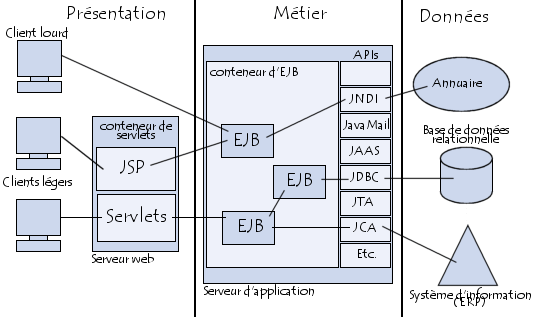
\includegraphics[scale=0.65]{architecture_JEE.png}
   	\caption{Diagramme issu de\url{architecture_JEE.png}}
    \label{reference1}
\end{figure}

Et dans la figure  \ref{reference1}\footnote{Diagramme issu de \url{}}
** image**
Construit sur la plateforme de Java 2 édition standard (Java SE), la plateforme Java EE ajoute les possibilités nécessaires pour fournir une plateforme complète, stable, sécurisée, et rapide de Java au niveau entreprise. 
Dans la mesure où J2EE s'appuie entièrement sur le Java, il bénéficie des avantages et inconvénients de ce langage, en particulier une bonne portabilité et une maintenabilité du code.\\
\newline
\indent
L'ensemble de l'infrastructure d'execution JavaEE est donc constitué de services (API) et spécifications tel que:
HTTP et HTTPS
Java Transaction API (JTA)
Remote Method Invocation/Internet Inter-ORB Protocol (RMI/IIOP)
Java Interface Definition Language (Java IDL)
Java DataBase Connectivity (JDBC)
Java Message Service (JMS)
Java Naming and Directory Interface (JNDI)
API JavaMail et JAF (JavaBeans Activation Framework)
Java API for XML Processing (JAXP)
Java EE Connector Architecture
Gestionnaires de ressources
Entreprise Java Beans (EJB)
Java Server Pages (JSP)
Servlet
Java API for XML Web Services (JAX-WS, anciennement JAX-RPC)
SOAP with Attachments API for Java (SAAJ)
Java API for XML Registries (JAXR)

Dans le cadre de notre application, seule une sous partie de ces composants nous ont été utile, tel que, notemment, les servelets, les JSP, JavaMail ou encore Jdbc avec hibernate, tel que décrit dans le point suivant.

De plus, l'architecture J2EE repose sur des composants distincts, interchangeables et distribués, ce qui signifie notamment :

qu'il est simple d'étendre l'architecture ;
qu'un système reposant sur J2EE peut posséder des mécanismes de haute-disponibilité, afin de garantir une bonne qualité de service ;
que la maintenabilité des applications est facilitée.

Pour interagir avec notre solveur d'une part, de la base de données d'autre part, et par


%% ==== avantages
java EE vs php vs .net vs python

%% === apprentissage
Ce fut nouveau mais xxx
Ca nous à permit d'apprender les outils et les techniques les plus recherchée actuelement 

\subsection{Hibernate}

Pour pouvoir communiquer avec notre base de donnée à partir de notre code java, on a commencé avec jdbc\footnote{Java Database connectivity} mais cela n'était pas suffisant et on s'est tourné ver Hibernate.

Hibernate est un framework libre, appellé framework de  "mapping objet-relationnel" ou encore de "persistance objet des données" (voir Figure \ref{reference2}). 
\begin{figure}[!h]
    \center
   	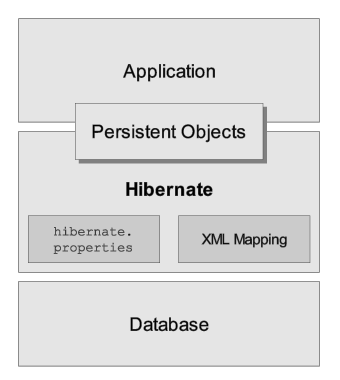
\includegraphics[scale=0.65]{schema_hibernate.png}
   	\caption{Diagramme issu de\url{}}
    \label{reference2}
\end{figure}
Ca permet donc à la couche applicative de notre programme de traiter les données vennant de la base de donnée comme des objects donc le contenu reste en mémoire même après la fin d'exécution du programme. D'où persistance objet des données. Le lien entre les classes exposées et la source physique des données (dans notre cas une base de données *relationnelle*) est définie par un fichier xml. D'où mapping objet-relationnel.
Cela nous à permit de gérer notre base de données, comme le reste de l'application en orienté objet, et même si son apprentissage ne fut pas des plus aisée, la gestion générale du code s'en est retrouvé grandement amélioré.

Un autre avantage recherché par cette solution, est que son indépendance à la base de donnée le rend ultra portable, et, sans aucune modification du code, notre application peu tourner sur 221\footnote{http://developers.sun.com/product/jdbc/drivers} base de données différente.  Notre application, après avoir configuré ses crédential dans le fichier de configuration d'Hibernate, se chargera de créer l'entièretée des tables et la structure de la base de donnée.

Théoriquement il aurait donc été possible d'envoyer directement un objet "hibernate" (représentant par exemple une table de notre bdd), à gwt, donc à l'utilisateur, malheureusement le monde n'est pas parfait, et comme stipulé dans la doc GWT\footnote{https://developers.google.com/web-toolkit/articles/using\_gwt\_with\_hibernate},
une SerializationException est levée à chaque fois un type transférée sur RPC n'est pas «sérialisable». La définition de la sérialisibilité signifie ici que le mécanisme RPC GWT sait comment sérialiser et désérialiser le type de bytecode au format JSON et vice-versa.
Le problème vient du fait qu'Hibernate modifie les objects afin de les rendre persistant (pour être exact, c'est la librairie javassist qui se charge de réécrire le bytecode de ces objects pour les rendre persistant). Au moment du transfer de l'object, une serialisation est tantée, mais n'étant pas le même (car modifé par javassist), il ne peut être sérialisé par RPC-GWTP.
Il a fallut donc rajouter des classes de type DTO\footnote{Data Transfer Object}, qui, eu sérialisable ont pu servir de communiquation entre la partie cliente et serveur.

Hibernate possedant sont propre language de requète HQL \footnote{Hibernate Query Language}, d'apparence similaire au SQL, mais pleinement orienté Object et comprenant des notions comme l'inheritance ou le polymorphisme\footnote{https://docs.jboss.org/hibernate/orm/3.3/reference/en/html/queryhql.html}.  Mais ca nous à bien fais chier (xx), et on a pas su en tirer pleinement avantage.



% chose qui interviennent dans la partie cliente et et serveur (gin/juice)
\section{Les outils client/serveur}

% organisation du code (avec des pseudo diagramme uml, explication local storage, rpc , % guice,...)
\section{Structure}

% schéma de la base de données (bdd de stockage)
% !TeX root = these.tex
\chapter{La base de données}

Avant de rentrer dans les détails de la base de données, il est a noter que la vision porté sur celle-ci doit être considéré différemment. L'utilisation d'Hibernate nous a permis de gérer la base de données de manière orienté objet et non plus d'une manière relationnel, la base de données n'est donc plus vue en tant que tel mais plutôt comme un ensemble de ces objets. Hibernate crée aussi des tables de mapping, et a sa propre façon de gérer le relationnelle.

La base de données se veut, délibérément, simple et minimale. Le but étant d'avant tout de manipuler les données liées aux attributions et aux autres données requises par la construction d'un horaire (désideratas, etc.). Nous avons donc évité de manipuler les informations superflus en important celles-ci statiquement dans la base de données. Notre application n'ayant pas pour objectif de modifier ces données.

Par exemple, nous ne nous soucions pas de données propre à l'année, la section, l'implantation, etc.,  Nous nous focalisons uniquement sur les attributions. Les informations qui les composes se doivent d'être séparées en différentes parties (par exemple, les professeurs, les différents groupes, etc.). Certaines données ne sont pas normalisées, ceci n'étant pas requis.

%Xavier, peux tu retravailler cette partie ;-)
Nous pouvons noter un objet plus particulier (correspondant donc à une table de la base de données), l'objet ActivityState. Celui-ci contient l'état d'un carton à un instant donné, c'est à dire, si ce carton est placé, à quel endroit et dans quel ordre le placement a été effectué.  Cette manière de faire nous permettra d'offrir un historique complet de ce qui a été fait en permettant des retours en arrière ou d'offrir une vision statistique de la construction de l'horaire. Nous privilégions de cette manière,  la rapidité et la facilité d'ajout (cette manière ne nécessitant pas de mettre le carton à jour) et prévient également les différentes erreurs pouvant survenir comme une écriture simultanée par différents utilisateurs au sein d'un même projet, d'une perte de connexion, etc.. Ceci étant des perspectives d'avenir du programme et n'étant pour le moment pas prisent en compte.

Afin de stoquer et manipuler les contraintes necessaire à notre application, nous avons décider de gérer ca d'une manière assez simple et intuitive. 
Le principe de base est de représenter une contrainte/désiderat par un tripplet <source-nivau-destination>.  La source pouvant être des professeurs, locaux, cours, cartons, groupe. Le niveau est simplement un nivau de préférence, qui permettra principalement de savoir si cette contrainte est du type "hard" ou "soft".  La destination est quand à elle soit une période de la semaine soit un local.  De cette manière, une grande partie des contraintes décrite au chapitre 1 peux être représenté.  Pour ce qui est des contraintes portant sur un ensemble (e.g. si on veut que tt les locaux du premier étage soient disponible le lundi matin, il suffira de mettre une contrainte sur chaqu'un de ses locaux du style <L42 - 3 - Lundi première heure>.  En pratique, on a représenté ca par un Objet( table) Préférence sur les diférente source possible.
Un autre type de contrainte peut être stoqué (bien qu'elle n'est pas encore réelement prise en compte), et la notion de dépendance entre 2 cartons.  Pour des cours qui doivent par exemple etre le plus éloigné ou le plus raproché possible.

Mais, on ne permet actuelement pas (et de tt facon, le solveur ne peut pas les gérer), toute les contraintes dépendante entre elles où conditionnelle (e.g. si le prof X ne peut pas avoir son jour de congé le lundi, il aimerait avoir ses matiné de libre ou ..)

Pour finir, nous dirons que la base de données n'est pas la base de données complète, celles-ci est très évolutive, étant donner les possibilités et facilités offertes par Hibernate.

% le solveur qu'on a choisi, comment ça marche
\section{Solveur}
le but ici n'est pas d'énumérer toutes les étapes par lesquelles nous sommes passé ainsi que toutes les essais infructué effectué, car ce serait long et inninteressant. Nous allons nous concentrer sur la méthode actuelle utilisée en tantant de justifié son choix. Pour pouvoir expliquer son choix et sont utilisation, nous allons devoir revenir sur les explications plus générale de la programmation par contraites et d'autre thechniques OR (operation research).  Pour plus d'information sur le sujet, nous invitons le lecteur, à XXX, ainsi qu'à la thèse de M qui fut de loins l'ouvrage qui nous a le plus éclairé quand la à la problematique de xx

Le solveur (celui du coté serveur), est indépendant de tout, absolument tout. Il est écrit en java, et repose sur une librérire de csp. Il réside donc du coté serveur, dans le servelet de l'application, c'est donc le meme pour tout utilisateurs se connectant au  site. Il ressevra l'information et l'enregistrera xxx


Apprès bpc de recherches, cette librairie est de loins la plus adapté et à jours (la dernière version datant du 20 juin, est d'ailleur celle utilisé par le programme).  Ca permetra un dévellopenment du solveur, independament de la bdd ou de l'interface.
Les possibilités de cette librairie combiné à nos choix d'infrastrcuture sont énorme, et à notre grande tristèsse, ne sont pas utilisé au maximum de sa puissance..  seule la surface à pu être implémenté, faute de temps.

----
Pour pouvoir apporter un réel avantage à notre application, comparé à la méthode actuelle, était de fournir une certaine "inteligence" à notre application.
Une partie de cette "inteligence" est pris en charge du coté client, qui comme décrit dans une précédente section, se charge d'assister l'utilisateur lors de la création de son horraire.

Cependant, ce support est minimaliste, et une recherche plus poussée est effectué du coté serveur à l'aide d'outil de programmation par contraite et de "recherche opérationnelle".

Pour comprendre notre choix de librairie ainsi que son utilisation, il est important de revenir sur les principe fondamentaux de la programmation par contraintes.


\subsection{Rappels théorique}

La programmation par contrainte un paradigme de programmation \footnote{paradigme} ayant pour but la résolution de problèmes combinatoire en
descrivant plutot le but recherché que la méthode utilisé, c'est pourquoi la programmation par contrainte es une forme de programmation déclarative.
--citation--

dans le cas qui nous concerne, la problème de création d'horraire, est un cas typique de CSP


% se trouve pour le moment, les differents chapitre de relexion
% concernant par ex la secu, la perf, etc
% !TeX root = these.tex
\chapter{Discussions}
\section{Choix concernant la performance}
\section{Choix concernant la sécurité}

Du fait de nos choix de conception, tel que gwt pour générer le java-script, ou
hibernate pour abstraire la base de donnée, ou le choix des rpc pour la
commnuniquation client-serveur,..  Nous pensons avoir créé une application ``de
base'', très sécure, et qu'il serait tout à fait envisageable de faire tourner notre
application sur un serveur externe.
(xxx) xss, csrf, sha256, check (basique) de la complexité du mot de passe, ainsi
qu'un catcha très basique aussi pour eviter des bots.

La secu du coté serveur à également été pris en compte, mais, logiquement, en
moins poussé (quoi que).  A savoir: l'application tourne sur une debian *stable*
(à savoir Squeeze), n'ayant que peu de services installé.
Tomcat, notre conteneur d'applet, est lui aussi à jours, et en version stable,
il ne bénificie d'aucun droit root, ainsi donc, (contrairement à une autre
application tournant sur Windows par exemple), il n'a pas le droit d'emmetre sur
le port 80. Pour garder l'application safe et peformante, une redirection de
son port d'origine est effectué par netfiller sur le port 80.

Nous avons pas poussé plus loins la sécu du coté serveur, étant donnée qu'elle
est destiné à fonctionner sur d'autre machine, mais en situation réel, il serait
jusdicieu de mettre en place un liens https.  En situation réel, nous
préconisons xxx (parfeu, strapping, vm,..)

N'étant pas infaillble, la mise à jour (très aisée pour notre type
d'application), est nous semple -t-il, une part importante dans la sécurité du
système. (cela probablement accentué par la mise de notre code source sous une
license ouverte (gpl3) )


% Comment nous avons travailler (gitHub, skype, egit,...)
% !TeX root = these.tex
\chapter{Méthodologie de conception}
Un programme informatique, comme n'importe quel projet, nécessite une bonne gestion pour pouvoir assurer un bon déroulement de ce projet.
D'une part, il faut faire face aux difficultés liées au travail d'équipe, d'autre part, il faut gérer le projet en tant que tel.

  \section{GIT et partage des données}
  La création d'un logiciel en équipe implique la gestion de cette équipe ainsi que le partage et l'échange des
  informations entre chaque membre de celle-ci.
  L'équipe doit travailler de façon coordonnée, elle doit s'échanger l'état
  d'avancement du travail ainsi que les résultats obtenus. Pour ce faire, il faut
  de bons moyens de communication, ou dans notre cas, UN bon moyen de communication: GIT\cite{git}. \\

  GIT est un logiciel de gestion de version décentralisé. Il permet de
  travailler à plusieurs sur un même projet. Il gère lui-même l'évolution du
  contenu en fusionnant les changements sans perte d'information. Il garde
  également en mémoire toutes les versions du code. Il est libre, gratuit et
  particulièrement facile à utiliser. Le code se trouve sur un dépôt internet, nous avons choisi GitHub\cite{github} pour ce dépôt.\\

  \section{Logiciel de suivi de problème}
  En plus de cette gestion de versions, GitHub offre un logiciel de suivi de problème, c'est-à-dire, un bugtracker.
  Un logiciel de suivi de problème est en quelque sorte un journal des problèmes classés par type.
  C'est un outil particulièrement utile pour le développement en équipe. Il donne un aperçu clair des bugs et de leurs états.

  \section{Méthodologie de conception}
Pour ce travail, il a été important d'avoir une méthode de travail rigoureuse. Nous avons donc scindé le travail en plusieurs parties, sous forme de bloques à effectuer. Pour chacun de ces bloques, nous avons noté les problèmes de conceptions, si il y en a eu, que nous avons pu rencontrer. Nous avons analyser comment chaque bloque pouvait etre conceptualiser, nous pouvons par exemple citer le filtre de cartons qui ne pouvais être conçu avec les outils de base proposé par GWT. Nous avons donc soigneusement analysé chaque partie avant de nous lancer tête baissé dans la conception d'un bloque pour ensuite se retrouver bloquer par les possibilités qui nous était offerte.

Nous avons suivit la méthode RUP\footnote{Rational Unified Process} basé sur UP, définissant un moyen de travailler sur des applications de type orienté objet. elle fournis de nombreux avantages comme le rôle de chaque acteur du projet, le cycle de vie de l'application, etc. Nous nous sommes donc basé sur cette méthode pour élaborer notre travail dans de bonne condition.

Nos besoins étant de trouver une méthode de travail en équipe et d'avoir une bonne gestion de projet. Nous ne rentrerons pas dans les détails de cette méthode, mais nous pouvons dire qu'elle nous à été bénéfique pour l'élaboration de notre application. Certain aspect de cette méthode comme la gestion de projets on pu directement être utiliser via GitHub et sont bugtracker. Cet outils nous a été d'une grande aide.

Nous avons conceptualiser notre application dans une optique d'extension. Dans cette objectif, rien n'a été fait statiquement afin de garantir l'évolution future de ce projet. C'est pour ces raisons que certains choix on été effectué, nous rendant la charge de travail plus lourde mais possédant des avantages non négligeable pour la bonne évolution de l'application. L'étendu et le potentiel d'un tel outil-logiciel est énorme, surtout pour un établissement scolaire, nous nous sommes donc conforté dans cette optique.
    
%        * mettre ici la façon dont vous avez \enquote{fait} le pgm* \\
%    
%    cad comment vous avez fait en pratique : on a ciblé nos besoins (citer les besoins) et nous nous sommes
%    dirigé vers le type de conception/méthodologie MACHIN(*mettre une référence*) qui consiste à faire de l'essai %erreur et être à la bourre 
%sans savoir où on va ni n'ou on vient. MAIS, comme on est pas des poulets, on a fait un planning. Le bugtracker nous a %également été très utile.
%
%Ce paragraphe n'est pas nécessaire, mais dans l'optique où votre promoteur aimera savoir ce que vous avez glandé %pendant l'année, c'est ici qu'il 
%faut lui prouver que 1> vous aviez une bonne méthodologie de travail (important) 2> vous avez pas glandé = pensé à tel %ou tel problème futur, telle ou telle option future, tel truc plus compliqué à faire mais qui permet ceci ou cela.
%Attention, QUE du blabla, rien de technique (vu qu'on l'explique que après)

% Amélioration envisagable pour le logiciel
\section{Amélioration future}

\subsection{Possibilités d'amélioration du programme}

\subsubsection{mode comparaison}
C'était un de nos objectifs principaux; il était question de pouvoir créer à la
voilée les collonnes représentant plusieur professeurs, loacux ou classe, tout
en gardant, pour les lignes, les périodes. Malheureusement le manque de temps à
eu raison de nous, ains qu'un problème fondamentale, à savoire qu'il n'es pas
possible, de rendre une région ne fesant pas partie du DOM (typiquement rajouté
en js, donc d'une manière non-statique) comme étant une région ``dropable''.
Cela n'étant certainement pas impossible, la solution idéal nous est pas encore
connue; probablement qui faudrait rendre l'entièreté de la région contenant le
tableau comme ``dropable'' afin de subdifiser celle ci.. car actuelement ce soit
les ``cases'' qui sont dropable..
\subsubsection{solveur}
Ce fu également un point assez frustrant, étant donné nos recheches abondante
sur le sujet, et surtout la trouvaille de cette librairire ``miraculeuse'' écrit
par Muller, et qui, en plus d'être en gpl et fortement maintenue (dernière
version date d'il y a 2 semaines), elle nous parrait très performante et d'une
rare adéquoicité.  C'est donc avec bcp de tristesse dans l'ame (:p), qu'on n'en
utilise qu'une fractions de ses possibilité.  C'était tout l'avantage de notre
application (et de sont architectur client-server) et ce n'est pas utilisé a son
full potentiel.  C'est donc la première amérioration que devra subir notre
application, car tout est en place pour pouvoir en tirer un avantage certain.
\subsubsection{droits}
Un des but de cette architecture était de pouvoir avoir plusieurs compte lié à
un projet, avec des droits différents, imaginons des professeurs qui pouraient
éditer leur désidérata, ou certaine parsonne qui pourait suivre l'évoltion de la
construction de l'horaire sans pour autant avoir les droits de modification.
\subsubsection{mode hors ligne}
On se base entièrement sur le local storage, les requètes vers le serveur ne
servent qu'a se connecter, charger le projet et enregistrer des modifications.
Actuelement, il est possible de continuer la création d'un horraire chargé en
mémoire sans la necessité d'une connections, cependant, pour pouvoir pleinement
utiliser cette fonctionnalité, il est necessaire de rajouter certaine xxx, tel
qu'une resyncronisation des modifications faite en local avec la bdd lors que la
connection est retrouvée ainsi que la possibilité de reprendre un projet en
cache.
\subsubsection{upload à partir d'une bdd}
\subsubsection{modifications de données}
actuelement il n'est pas possible de modifier toutes les données intervenant
dans l'application (notament la création d'un prof, local, etc), 


% nos recommandation sur l'utilisation, le fichier xls,...
% !TeX root = these.tex
\chapter{Recommandation}

% !TeX root = these.tex
\chapter*{Conclusion}

Dans le présent rapport, nous avons vu comment répondre au problème réel et récurrent de la création d'horaires dans le contexte académique. Pour répondre à cette problématique, nous avons dû effectuer un large travail sur trois quatre aspects en particuliers ; la programmation par contraintes, une solution client/serveur, et, enfin, un travail collaboratif en équipe.\\
\newline
\indent
Dans le cadre de la programmation par contraintes, un travail a été fait sur la théorie sous-jacente aux contraintes et au paradigme de programmation correspondant. Cet aspect a été travaillé tant dans la littérature sur le sujet que lors de notre rencontre avec Monsieur  \textsc{Schaus}, docteur dans le sujet.
Cette rencontre a notamment souligné l'importance du choix des bons outils. En effet, il existe de nombreuses librairies dédiées à la programmation par contraintes, cependant peu sont adaptées à notre problème et permettent de prendre en compte la pondération des contraintes. En effet, comme évoqué précédemment, un \textit{desiderata} exprimé par un professeur n'est pas vraiment une contrainte dure et doit être l'objet d'un traitement à l'aide de règles heuristiques et métaheuristiques.
\newline
\indent
Notre travail sur la programmation par contraintes nous a permis de théorisé plus facilement le problème posé par la création d'horaires à l'EPHEC. Rappelons que ce problème a été analysé notamment grâce à notre entretien avec Madame \textsc{Gillet}, directrice de l'établissement sur le site de Louvain-la-Neuve.
En définitive, nous avons utilisé les libraires offertes par \textit{UniTime} afin d'implémenter un solveur permettant de résoudre les problèmes posés par la création d'horaire.\\
\newline
\indent
Cependant, afin de rendre notre solution utile au plus grand nombre, il a été choisi de prendre une architecture client/serveur. Cette architecture permet notamment de minimiser les problèmes classiques côté client, de centraliser les données sur un seul serveur et d'utiliser des technologies fiables.
En outre, en utilisant GWT, nous avons permis de scinder l'exécution du code entre le serveur et le client. En effet, comme expliqué précédemment, GWT permet de transposer du Java en JavaScript afin de faire exécuter le code par le navigateur côté client.
\newline
\indent
Enfin, nous avons privilégié les derniers standards, tels que HTML5 et CSS3, afin d'assurer une compatibilité ascendante dans le développement futur de l'application.
Ainsi, cet aspect client/serveur permet d'élaborer une interface Web afin de permettre à l'utilisateur de se concentrer sur l'aspect important de sa tâche, à savoir la création d'horaire.\\
\newline
\indent
Nous avons réalisé cette solution en équipe. Cet aspect a nécessité d'utiliser certaines méthodes et certains outils. Ces derniers sont surtout git et les systèmes de téléphonie VIP. Ce travail en équipe nous a permis d'apprendre à travailler en équipe et de mettre au point des normes de codage.\\
\newline
\indent
Plus personnellement, ce travail nous a particulièrement tenu à cœur. En effet, beaucoup de travail a été fourni pour utiliser des technologies modernes tels que Hibernate, Java EE que nous pensons être des atouts dans le monde professionnel. Toutefois, il est nécessaire de souligner que nous avons été surpris par la longueur d'apprentissage et d'implémentation de ces technologies. Ces difficultés ont dû être analysées et réglées, notamment au niveau problématique de la gestion asynchrone des échanges client et serveur.
\newline
\indent
En effet, bien que la solution que nous proposons soit encore perfectible en de nombreux points, notamment au niveau des résolutions de contraintes complexes qui étaient l'objectif premier de ce travail, il est nécessaire de souligner que la méthodologie ayant conduit à son élaboration et les choix technologiques pris permettent, malgré la grande quantité de code, une maintenabilité et une robustesse relatives.
\newline
\indent
De plus, la méthodologie suivie, qui consistait à découper les parties du projets en blocs, aurait permis de doubler l'équipe sans que les différents développeurs aient à se marcher sur les pieds. De plus, les moyens mis en place pour développer la solution de façon collaborative auraient permis la gestion d'une équipe plus grande.\\
\newline
\indent
En conclusion, nous avons proposés une méthodologie ainsi qu'une solution pour l'assistance à la création d'horaire. Cet aspect rejoint le domaine plus large de la recherche opérationnelle dans laquelle s'inscrit ce présent projet. 





\backmatter

\newpage
\bibliography{official}
\bibliographystyle{apalike-fr}

%\newpage
%\listoffigures
%
%\newpage
%\listoftables

\renewcommand{\thesection}{\Alph{section}}
\setcounter{section}{0} 

%% !TeX root = these.tex
\newpage
\chapter*{Annexes}

\setcounter{page}{1}
\pagenumbering{roman}
%\pagenumbering{Roman}
%\pagenumbering{Arabic}



\section{Formats de sérialisation RDF}
\label{annexe/serialisation}

% Pour les citer, voir Annexe \ref{annexe/serialisation}
% Important : compiler 2x

%\begin{figure}[!h]
%    \center
%   	\includegraphics[scale=0.75]{figureX.png}
%\end{figure}



\newpage


\section{Exemple de code}
\label{annexe/espace_nom}

\begin{figure}[!h]
\begin{lstlisting}[frame=single]
 from constraint import *
 problem = Problem()
 problem.addVariable("a", [1,2,3])
 problem.addVariable("b", [4,5,6])
 problem.getSolutions()
[{'a': 3, 'b': 6}, {'a': 3, 'b': 5}, {'a': 3, 'b': 4},
 {'a': 2, 'b': 6}, {'a': 2, 'b': 5}, {'a': 2, 'b': 4},
 {'a': 1, 'b': 6}, {'a': 1, 'b': 5}, {'a': 1, 'b': 4}]

 problem.addConstraint(lambda a, b: a*2 == b,
                          ("a", "b"))
 problem.getSolutions()
[{'a': 3, 'b': 6}, {'a': 2, 'b': 4}]

 problem = Problem()
 problem.addVariables(["a", "b"], [1, 2, 3])
 problem.addConstraint(AllDifferentConstraint())
 problem.getSolutions()
[{'a': 3, 'b': 2}, {'a': 3, 'b': 1}, {'a': 2, 'b': 3},
 {'a': 2, 'b': 1}, {'a': 1, 'b': 2}, {'a': 1, 'b': 3}]
\end{lstlisting}
\caption{Code python}
\end{figure}

\newpage


\section{Page de connexion et d'inscription}
\label{annexe/espace_nom}

\begin{figure}[!h]
	\begin{center}
		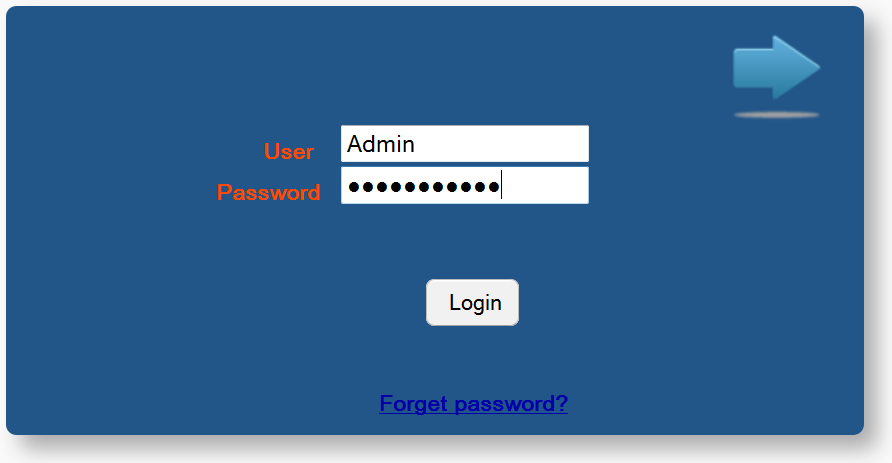
\includegraphics[width=16cm,height=8cm]{login.png}	
		\caption{page de connexion}
	\end{center}
\end{figure}

\begin{figure}[!h]
	\begin{center}
		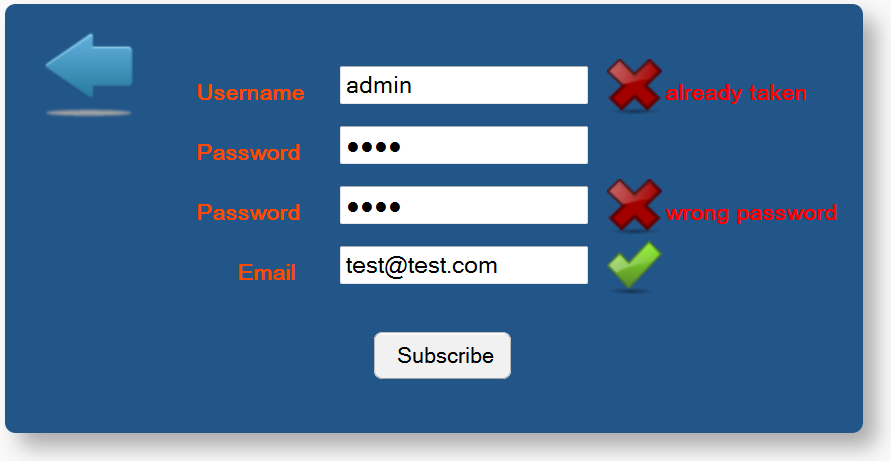
\includegraphics[width=16cm,height=8cm]{subscribe.png}
		\caption{page d'inscription}
	\end{center}
\end{figure}

\newpage

\section{Page des projets}
\label{annexe/espace_nom}

\begin{figure}[!h]
	\begin{center}
		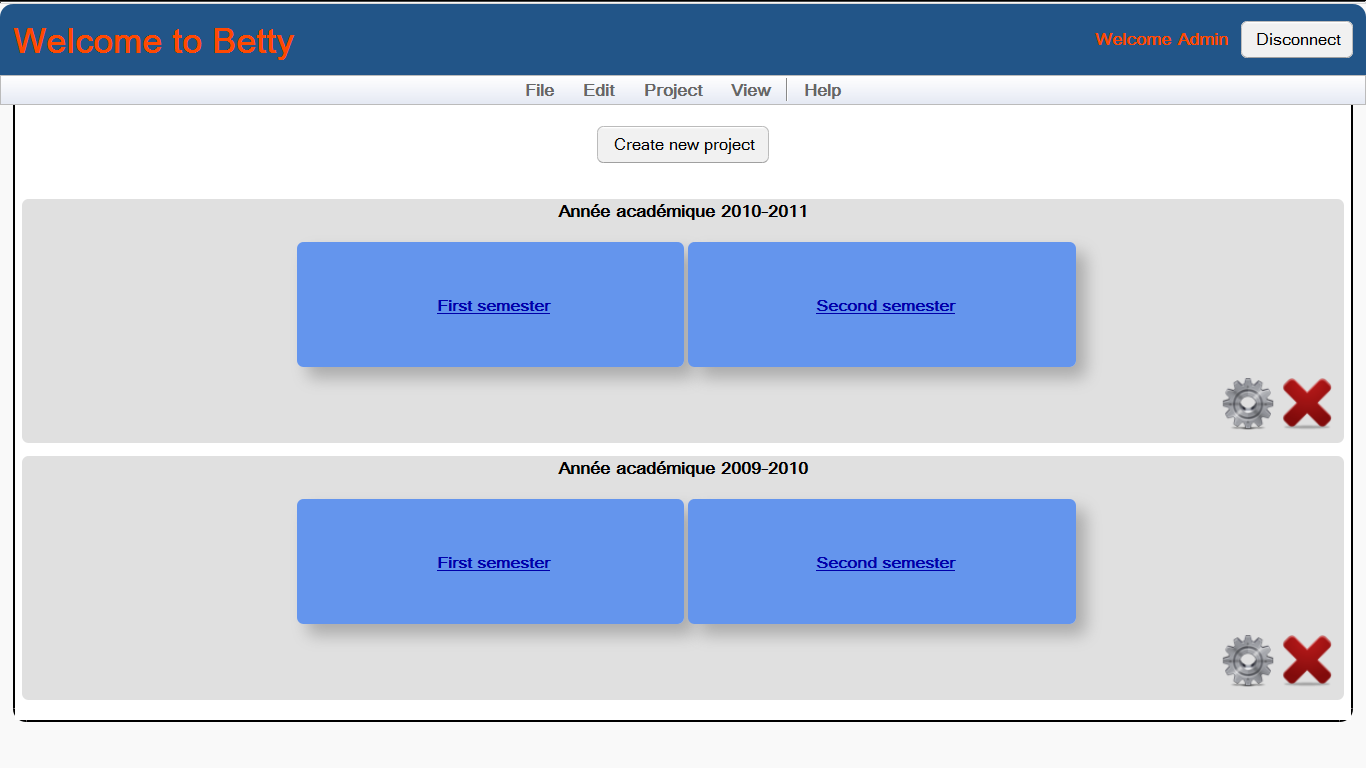
\includegraphics[width=19cm,height=12cm,angle=90]{ProjectPage.png}
		\caption{page des projets}
	\end{center}
\end{figure}\newpage

\newpage

\section{Page principale I}
\label{annexe/espace_nom}

\begin{figure}[!h]
	\begin{center}
		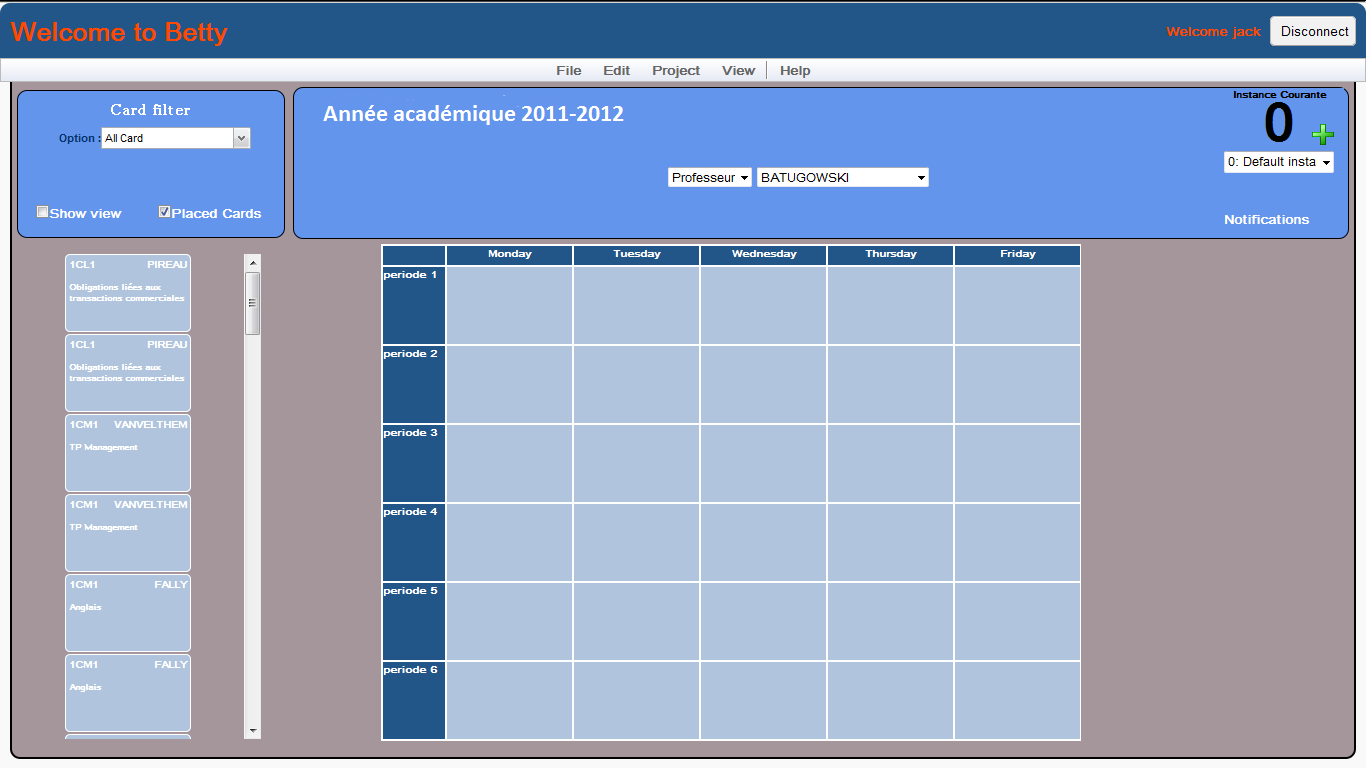
\includegraphics[width=19cm,height=12cm,angle=90]{MainPageClean.png}
		\caption{page principale vide}
	\end{center}
\end{figure}

\newpage

\section{Page principale II}
\label{annexe/espace_nom}

\begin{figure}[!h]
	\begin{center}
		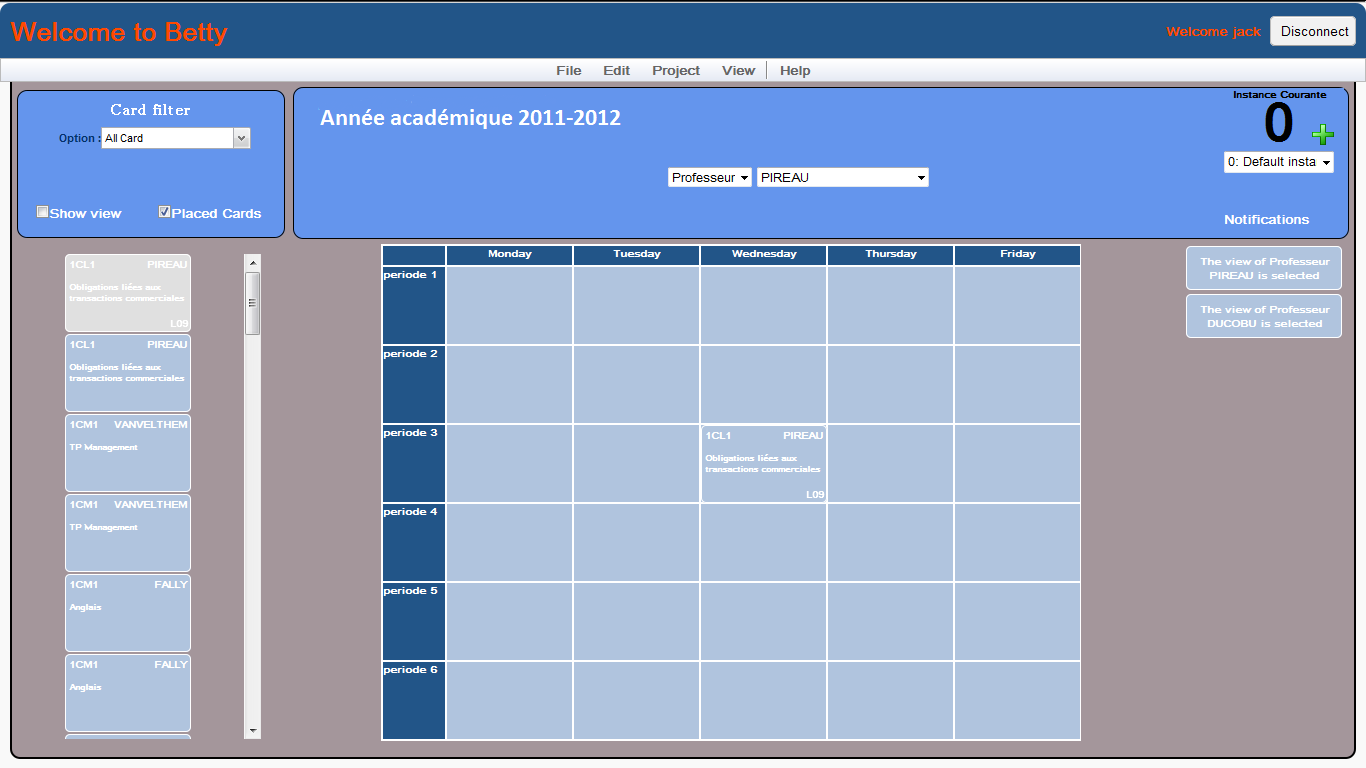
\includegraphics[width=19cm,height=12cm,angle=90]{MainPagePlacedCard.png}
		\caption{page principale carton placé}
	\end{center}
\end{figure}

\newpage

\section{Page principale III}
\label{annexe/espace_nom}

\begin{figure}[!h]
	\begin{center}
		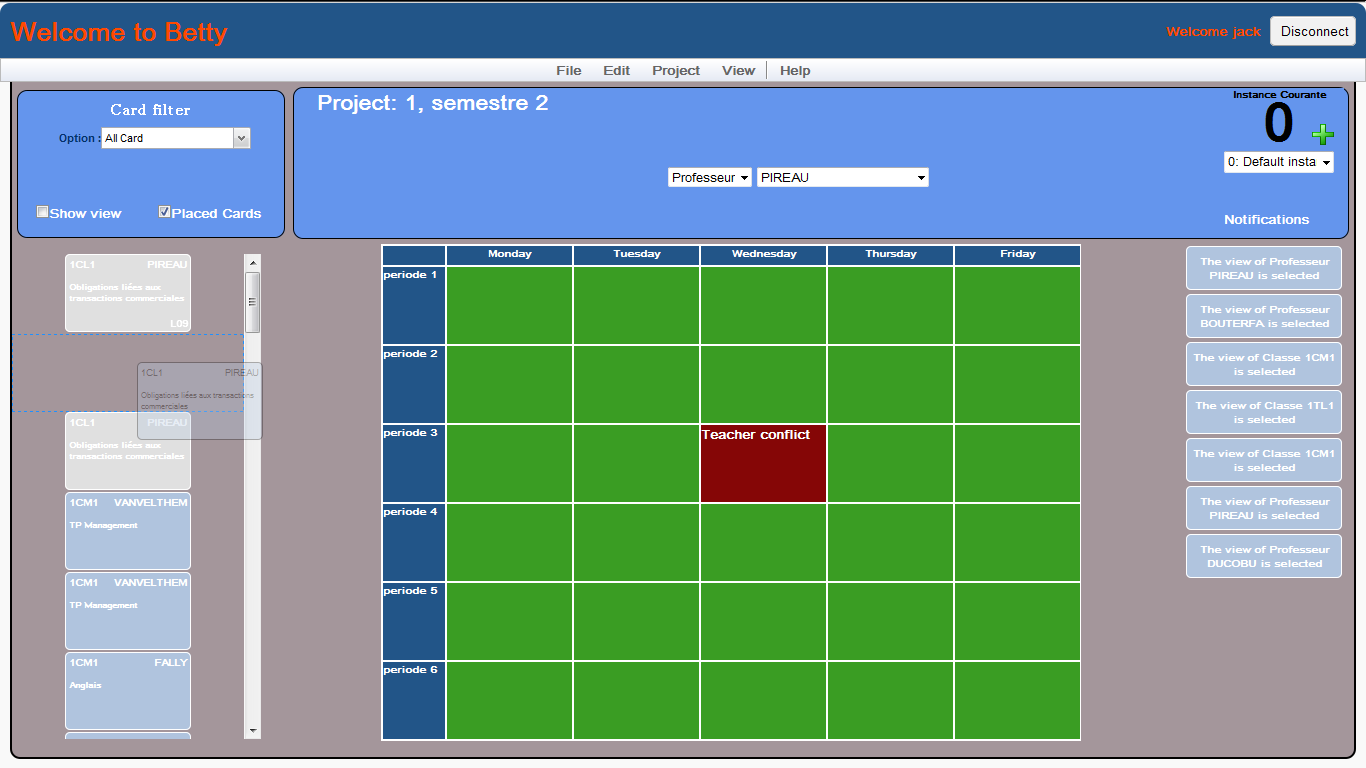
\includegraphics[width=19cm,height=12cm,angle=90]{MainPageColorTab.png}
		\caption{page principale solveur client}
	\end{center}
\end{figure}

\newpage

\section{Card filter}
\label{annexe/espace_nom}

\begin{figure}[!h]
	\begin{center}
		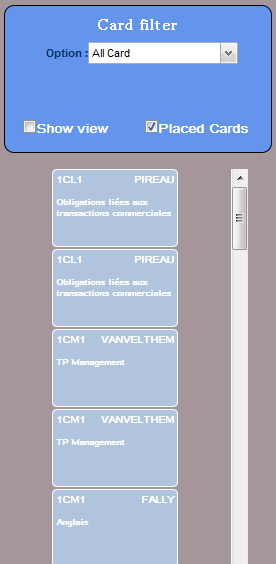
\includegraphics[width=6cm,height=12cm]{CardFilterAllCard.png}
		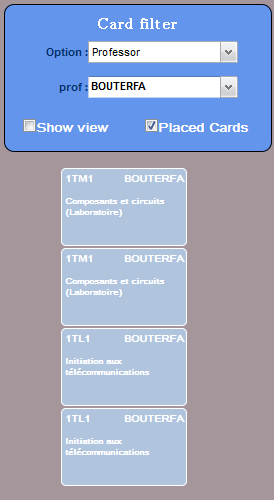
\includegraphics[width=6cm,height=10cm]{CardFilterBouterfa.png}
		\caption{présentation des cartons (non) filtrés}		
		\includegraphics[width=6cm,height=8cm]{CardFilterChoice.png}
		\caption{filtre avec multi-sélection}
	\end{center}
\end{figure}




%\makeback
\end{document}
